\documentclass[11pt,openany]{article}

\usepackage{mathtools, commath}
% Packages for formatting
\usepackage[margin=1in]{geometry}
\usepackage{fancyhdr}
\usepackage{enumerate}
\usepackage{graphicx}
\usepackage{kotex}
\usepackage{arydshln} % Include this package
\usepackage{bbding}
\usepackage{amsmath}
\usepackage{amsthm}
\usepackage[dvipsnames,table]{xcolor}
\usepackage{amssymb, amsfonts}
\usepackage{wasysym}
\usepackage{footnote}
\usepackage{tablefootnote}
\usepackage{arydshln} % Include this package

% Fonts
\usepackage[T1]{fontenc}
\usepackage[utf8]{inputenc}
\usepackage{newpxtext,newpxmath}
\usepackage{sectsty}

% Define colors
\definecolor{TealBlue1}{HTML}{0077c2}
\definecolor{TealBlue2}{HTML}{00a5e6}
\definecolor{TealBlue3}{HTML}{b3e0ff}
\definecolor{TealBlue4}{HTML}{00293c}
\definecolor{TealBlue5}{HTML}{e6f7ff}

\definecolor{thmcolor}{RGB}{231, 76, 60}
\definecolor{defcolor}{RGB}{52, 152, 219}
\definecolor{lemcolor}{RGB}{155, 89, 182}
\definecolor{corcolor}{RGB}{46, 204, 113}
\definecolor{procolor}{RGB}{241, 196, 15}

\usepackage{color,soul}
\usepackage{soul}
\newcommand{\mathcolorbox}[2]{\colorbox{#1}{$\displaystyle #2$}}
\usepackage{cancel}
\newcommand\crossout[3][black]{\renewcommand\CancelColor{\color{#1}}\cancelto{#2}{#3}}
\newcommand\ncrossout[2][black]{\renewcommand\CancelColor{\color{#1}}\cancel{#2}}

\usepackage{hyperref}
\usepackage{booktabs}

% Chapter formatting
\definecolor{titleTealBlue}{RGB}{0,53,128}
\usepackage{titlesec}
\titleformat{\section}
{\normalfont\sffamily\Large\bfseries\color{titleTealBlue!100!gray}}{\thesection}{1em}{}
\titleformat{\subsection}
{\normalfont\sffamily\large\bfseries\color{titleTealBlue!50!gray}}{\thesubsection}{1em}{}

%Tcolorbox
\usepackage[most]{tcolorbox}
\usepackage{multirow}
\usepackage{multicol}
\usepackage{blindtext}

\usepackage[linesnumbered,ruled]{algorithm2e}
\usepackage{algpseudocode}
\usepackage{setspace}
\SetKwComment{Comment}{/* }{ */}
\SetKwProg{Fn}{Function}{:}{end}
\SetKw{End}{end}
\SetKw{DownTo}{downto}

% Define a new environment for algorithms without line numbers
\newenvironment{algorithm2}[1][]{
	% Save the current state of the algorithm counter
	\newcounter{tempCounter}
	\setcounter{tempCounter}{\value{algocf}}
	% redefine the algorithm numbering (remove prefix)
	\renewcommand{\thealgocf}{}
	\begin{algorithm}
	}{
	\end{algorithm}
	% Restore the algorithm counter state
	\setcounter{algocf}{\value{tempCounter}}
}

\usepackage{adjustbox}
% Header and footer formatting
\pagestyle{fancy}
\fancyhead{}
\fancyhf{}
\rhead{\textcolor{TealBlue2}{\large\textbf{리만의 복소해석을 토대로 얻는 내 수학적 시야 (2기)}}}%\rule{3cm}{0.4pt}}
\lhead{\textcolor{TealBlue2}{\large\textbf{수학의 즐거움, Enjoying Math}}}
% Define footer
%\newcommand{\footer}[1]{
%\begin{flushright}
%	\vspace{2em}
%	\includegraphics[width=2.5cm]{school_logo.jpg} \\
%	\vspace{1em}
%	\textcolor{TealBlue2}{\small\textbf{#1}}
%\end{flushright}
%}
%\rfoot{\large Department of Information Security, Cryptogrphy and Mathematics, Kookmin Uni.\includegraphics[height=1.5cm]{school_logo.jpg}}
\fancyfoot{}
\fancyfoot[C]{-\thepage-}

\usepackage{animate}
% Load the PDF and grab its total pages into \NumPages:
\newcount\NumPagesA
\pdfximage{../riemann-tikz/secant_line_gif.pdf}% loads the PDF
\NumPagesA=\pdflastximagepages
\usepackage{tcolorbox}
\tcbset{colback=white, arc=5pt}

\definecolor{axiomcolor}{HTML}{a88bfa}
\definecolor{defcolor}{RGB}{52, 152, 219}
\definecolor{procolor}{RGB}{241, 196, 15}
\definecolor{thmcolor}{RGB}{231, 76, 60}
\definecolor{lemcolor}{RGB}{155, 89, 182}
\definecolor{corcolor}{RGB}{46, 204, 113}
\definecolor{execolor}{RGB}{90, 128, 127}

% Define a new command for the custom tcolorbox
\newcommand{\axiombox}[2][]{%
	\begin{tcolorbox}[colframe=axiomcolor, title={\color{white}\bfseries #1}]
		#2
	\end{tcolorbox}
}

\newcommand{\defbox}[2][]{%
	\begin{tcolorbox}[colframe=defcolor, title={\color{white}\bfseries #1}]
		#2
	\end{tcolorbox}
}

\newcommand{\probox}[2][]{%
	\begin{tcolorbox}[colframe=procolor, title={\color{white}\bfseries #1}]
		#2
	\end{tcolorbox}
}

\newcommand{\thmbox}[2][]{%
	\begin{tcolorbox}[colframe=thmcolor, title={\color{white}\bfseries #1}]
		#2
	\end{tcolorbox}
}

\newcommand{\lembox}[2][]{%
	\begin{tcolorbox}[colframe=lemcolor, title={\color{white}\bfseries #1}]
		#2
	\end{tcolorbox}
}
\usepackage{amsthm}

% Define custom theorem styles
\newtheoremstyle{dotless} % Name of the style
{3pt} % Space above
{3pt} % Space below
{\itshape} % Body font
{} % Indent amount
{\bfseries} % Theorem head font
{} % Punctuation after theorem head
{2.5mm} % Space after theorem head
{} % Theorem head spec

\newtheoremstyle{definitionstyle} % Name of the style
{3pt} % Space above
{3pt} % Space below
{} % Body font
{} % Indent amount
{\bfseries} % Theorem head font
{.} % Punctuation after theorem head
{2.5mm} % Space after theorem head
{} % Theorem head spec

% Applying custom styles
%\theoremstyle{dotless}
\newtheorem{theorem}{Theorem} % Theorem environment with section-wise numbering
\newtheorem*{theorem*}{Theorem} % Theorem environment with section-wise numbering
\newtheorem*{lemma*}{Lemma} % Theorem environment with section-wise numbering
\newtheorem*{proposition*}{Proposition} % Theorem environment with section-wise numbering
\newtheorem*{corollary*}{Corollary} % Theorem environment with section-wise numbering
\newtheorem{proposition}[theorem]{Proposition} % Theorem environment with section-wise numbering
\newtheorem{lemma}[theorem]{Lemma} % Lemma shares the counter with theorem
\newtheorem{corollary}[theorem]{Corollary} % Corollary shares the counter with theorem

\theoremstyle{definitionstyle}
\newtheorem*{observation}{\textcolor{magenta}{Observation}}
\newtheorem*{illustration}{\textcolor{teal}{Illustration}}
\newtheorem*{torus}{{\color{red}T}{\color{orange}o}{\color{green!75!black}r}{\color{cyan}u}{\color{violet}s}}
\newtheorem{definition}{Definition} % Definition shares the counter with theorem
\newtheorem{example}{Example} % Example shares the counter with theorem
\newtheorem{exercise}{{Exercise}} % Example shares the counter with theorem
\newtheorem{remark}{Remark} % Remark shares the counter with theorem
\newtheorem*{note}{Note}
\newtheorem*{notation}{Notation}

\newtheorem*{axiom*}{Axiom}
\newtheorem*{definition*}{Definition} % Definition shares the counter with theorem
\newtheorem*{example*}{Example} % Example shares the counter with theorem
\newtheorem*{exercise*}{\textcolor{teal}{Exercise}} % Example shares the counter with theorem
\newtheorem*{remark*}{Remark} % Remark shares the counter with theorem


\usepackage{tikz}
\usepackage{tikz-cd}
\usetikzlibrary{shadows}
\usetikzlibrary{shapes.geometric, arrows.meta, positioning}
\input{riemann-complex-commands}
\renewcommand{\vec}[1]{\mathbf{#1}}
\renewcommand{\emph}[1]{\textbf{#1}}
\renewcommand{\d}{\mathrm{d}} % For the exterior derivative 'd'
\newcommand{\pderiv}[2]{\frac{\partial #1}{\partial #2}}
\newcommand{\spderiv}[3]{\frac{\partial^2 #1}{\partial #2\partial #3}}
\newcommand{\vect}[1]{\begin{bmatrix} #1 \end{bmatrix}}

\newcommand{\circulationsquare}[1]{
	\draw[thick, gray] #1 rectangle ++(1,1);
	\begin{scope}[decoration={markings, mark=at position 0.5 with {\arrow{>}}}]
		\draw[postaction={decorate}, blue] #1 -- ++(1,0);
		\draw[postaction={decorate}, blue] ++(1,0) -- ++(0,1);
		\draw[postaction={decorate}, blue] ++(0,1) -- ++(-1,0);
		\draw[postaction={decorate}, blue] ++(-1,0) -- cycle;
	\end{scope}
}

\usepackage{esvect}
\usepackage{physics}

\setstretch{1.25}

\begin{document}
\pagenumbering{arabic}
\begin{center}
%	\huge\textbf{Riemann; Complex Analysis}\\
	\huge\textbf{From Vector Calculus to Differential Forms}\\
%	\Large - HW1 -\\
	\vspace{0.5em}
	\large{Ji, Yong-hyeon}\\
%	\large{\ttfamily \url{https://github.com/Hacker-Code-J}}\\
	\vspace{0.5em}
	\normalsize{\today}\\
\end{center} 
%\[\boxed{
%\underbrace{f}_{\Omega^0}
%\;\xrightarrow{d}\;
%\underbrace{df}_{\Omega^1}
%\;\longleftrightarrow\;
%\underbrace{\nabla f}_{\substack{\text{gradient}\\\text{vector field}}}
%\quad
%\longrightarrow
%\quad
%\underbrace{\mathbf F}_{(\Omega^0)^m}
%\;\xrightarrow{d}\;
%\underbrace{d\mathbf F}_{\Omega^1\otimes\R^m}
%\;\longleftrightarrow\;
%\underbrace{D\mathbf F}_{\substack{\text{Jacobian}\\\text{matrix}}}}
%\]
\noindent 
We cover the following topics in this note.
\begin{itemize}
	\item Vector calculus (conservative fields, irrotational field)
	\item Differential forms (exact forms, closed forms)
\end{itemize}
%In this note, we build a bridge between the familiar concepts of vector calculus (conservative fields, curl) and the language of differential forms (exact forms, closed forms)
%\hrule\vspace{12pt}
\begin{center}
	\begin{tabular*}{\textwidth}{@{\extracolsep{\fill}} l c l}
		\hline
		\textbf{Vector Calculus (in $\R^2$ or $\R^3$)} & & \textbf{Differential Forms} \\
		\hline
		Vector Field $\vec F$ & $\iff$ & 1-form $\omega$ \\
		Conservative Vector Field ($\vec F = \nabla f$) & $\iff$ & Exact 1-form ($\omega = \d f$) \\
		Irrotational Vector Field ($\nabla \times \vec F = \mathbf{0}$) & $\iff$ & Closed 1-form ($\d\omega = 0$) \\
		\hline
	\end{tabular*}
\end{center}

\vspace{1em}

\begin{framed}
	\noindent\textbf{The Fundamental Implication:}
	\begin{itemize}
		\item \textbf{Conservative $\implies$ Irrotational},\; i.e.,\; \textbf{Exact $\implies$ Closed}\\ (This is always true.)
		\item \textbf{Irrotational $\implies$ Conservative},\; i.e,\; \textbf{Closed $\implies$ Exact}\\ (This is only true on ``nice'' domains, e.g., simply connected ones.)
	\end{itemize}
\end{framed}


\tableofcontents
\newpage

\section{Conservative and Exact}
\subsection*{Why do we think of the ``Conservative Field (or Gradient Field)''?}

%\begin{tikzpicture}
%	\begin{groupplot}[
%		group style={group size=2 by 1, horizontal sep=2.2cm},
%		width=9cm, height=8cm,
%		xmin=-2, xmax=2, ymin=-2, ymax=2,
%		domain=-2:2, y domain=-2:2,
%		colormap/viridis,
%		axis on top,
%		]
%		
%		% --- Panel 1: Heatmap of f with gradient field arrows (top-down view) ---
%		\nextgroupplot[
%		title={Scalar field $f(x,y)=x^2+y^2$ with $\nabla f$},
%		view={0}{90},
%		axis equal image,
%		xlabel={$x$}, ylabel={$y$},
%		ticks=none,
%		]
%		% Heatmap (top-down view of the surface)
%		\addplot3[
%		surf, shader=interp,
%		samples=45, samples y=45,
%		] {x^2 + y^2};
%		
%		% Gradient field arrows: (2x, 2y)
%		\addplot3[
%		-stealth,
%		quiver={
%			u=2*x, v=2*y, w=0,
%			scale arrows=0.12
%		},
%		samples=16,
%		samples y=16,
%		domain=-1.8:1.8, y domain=-1.8:1.8,
%		] ({x},{y},{0});
%		
%		% --- Panel 2: 3D surface z = f(x,y) ---
%		\nextgroupplot[
%		title={$z=f(x,y)=x^2+y^2$ (surface)},
%		view={-35}{30},
%		xlabel={$x$}, ylabel={$y$}, zlabel={$z$},
%		samples=45, samples y=45,
%		zmin=0,
%		ticks=none,
%		]
%		\addplot3[
%		surf, shader=interp
%		] {x^2 + y^2};
%		
%	\end{groupplot}
%\end{tikzpicture}

\begin{center}
\begin{tikzpicture}
	\draw[-Stealth] (7,4) -- ++ (1,0) node[midway, above] {$\nabla=\left(\pderiv{}{x}, \pderiv{}{y}\right)$};
	\begin{groupplot}[
		group style={group size=2 by 1, horizontal sep=2.2cm},
		width=9cm, height=8cm,
		xmin=-2, xmax=2, ymin=-2, ymax=2,
		domain=-2:2, y domain=-2:2,
		colormap/viridis,
		axis on top,
		]
		% --- Panel 1: Heatmap of f with gradient field arrows (top-down view) ---
		\nextgroupplot[
		title={Scalar field $f(x,y)=x^2+y^2$},
		view={0}{90},
		axis equal image,
		xlabel={$x$}, ylabel={$y$},
		ticks=none,
		]
		% Heatmap (top-down view of the surface)
		\addplot3[
		surf, shader=interp,
		samples=45, samples y=45,
		colormap/cool
		] {x^2 + y^2};
		
		% --- Panel 2: 3D surface z = f(x,y) ---
		\nextgroupplot[
		title={Gradient field $\nabla f=\langle 2x,2y\rangle$},
		view={0}{90},
		axis equal image,
		xlabel={$x$}, ylabel={$y$},
		ticks=none,
		]		
		% Gradient field arrows: (2x, 2y)
		\addplot3[
		-stealth,
		quiver={
			u=2*x, v=2*y, w=0,
			scale arrows=0.12
		},
		samples=16,
		samples y=16,
		domain=-1.8:1.8, y domain=-1.8:1.8,
		] ({x},{y},{0});
	\end{groupplot}
\end{tikzpicture}
\end{center}
A vector field $\vec F$ is \textbf{conservative} if it is the \textbf{gradient}\footnote{Gradient is a measure of change in a scalar field} of some scalar potential function $f$: \[
\vec F = \nabla f=\begin{cases}
	\left\langle\frac{\partial f}{\partial x}, \frac{\partial f}{\partial y} \right\rangle &\text{ if}\; f:U(\subseteq\R^2)\to\R\\
	\left\langle\frac{\partial f}{\partial x}, \frac{\partial f}{\partial y}, \frac{\partial f}{\partial z}\right\rangle &\text{ if}\; f:U(\subseteq\R^3)\to\R\\
	\left\langle\frac{\partial f}{\partial x_1}, \frac{\partial f}{\partial x_2},\dots, \frac{\partial f}{\partial x_n}\right\rangle &\text{ if}\; f:U(\subseteq\R^n)\to\R
\end{cases}.
\] If $\vec F$ is conservative, line integrals only depend on the endpoints: \[
\int_{\gamma}\vec F\cdot \d\vec r= \int_{\gamma}\nabla f\cdot \d\vec r=f(\textrm{end}) - f(\textrm{start}),
\] which turns \textcolor{red}{hard line integrals} into \textcolor{blue}{simple evaluations}. Furthermore every closed loop (start = end) has integral $0$.

Equivalently (on a nice domain) every line integral of $\vec F$ is path-independent: \[
\int_{\gamma_1}\vec F\cdot \d\vec r = \int_{\gamma_2}\vec F\cdot \d\vec r.
\] whenever $\gamma_1$ and $\gamma_2$ have the same endpoints.

\newpage
\begin{center}
\begin{tikzpicture}[scale=1.4]
	% Axes
	\draw[->] (-2.4,0) -- (2.6,0) node[below right] {$x$};
	\draw[->] (0,-2.4) -- (0,2.6) node[above left] {$y$};
	
	% Level sets of f(x,y)=x^2+y^2 (circles)
	\foreach \r/\lab in {0.7/{0.49},1.2/{1.44},1.7/{2.89},2.2/{4.84}}{
		\draw[thin] (0,0) circle (\r);
	}
	\node[font=\scriptsize,align=left] at (1.9,1.85)
	{$f(x,y)=x^2+y^2$\\[-1pt](level sets are circles)};
	
	% Gradient field \nabla f = <2x,2y>
	\def\scale{0.18}
	\foreach \x in {-2,-1.5,...,2}{
		\foreach \y in {-2,-1.5,...,2}{
			\pgfmathsetmacro{\ux}{2*\x*\scale}
			\pgfmathsetmacro{\uy}{2*\y*\scale}
			\draw[-{Stealth[length=2mm]}, line width=0.28pt, opacity=0.9]
			(\x,\y) -- ++(\ux,\uy);
		}
	}
	\node[font=\scriptsize] at (-1.95,-1.85) {$\nabla f=\langle 2x,2y\rangle$};
	
	% Endpoints A and B
	\coordinate (A) at (-1.4,0.6);
	\coordinate (B) at (1.5,1.2);
	\fill (A) circle (1.4pt) node[above left] {$A$};
	\fill (B) circle (1.4pt) node[above right] {$B$};
	
	% Path gamma_1: straight segment A -> B
	\draw[
	very thick, blue!70,
	-{Stealth[length=2.4mm]},
	postaction={decorate},
	decoration={markings, mark=at position 0.5 with {\node[fill=white, inner sep=1pt, font=\scriptsize] {$\gamma_1$};}}
	] (A) -- (B);
	
%	% Path gamma_2: a curvy path A -> B (via a small arc then a bend)
%	\path let \p1=(A) in coordinate (C) at (-0.2,1.8);
%	\draw[
%	very thick, red!70!black,
%	-{Stealth[length=2.4mm]},
%	postaction={decorate},
%	decoration={markings, mark=at position 0.55 with {\node[fill=white, inner sep=1pt, font=\scriptsize] {$\gamma_2$};}}
%	] (A) to[out=60,in=210] (C) to[out=-30,in=180] (B);
	
%	% Annotations of endpoint values
%	\draw[dashed, gray!70] (A) -- (0,0);
%	\draw[dashed, gray!70] (B) -- (0,0);
%	\node[font=\scriptsize, align=left, fill=white, inner sep=1pt]
%	at ($(A)!0.65!(0,0)+(-0.35,-0.15)$)
%	{$f(A)=\|A\|^2$};
%	\node[font=\scriptsize, align=left, fill=white, inner sep=1pt]
%	at ($(B)!0.5!(0,0)+(0.35,-0.15)$)
%	{$f(B)=\|B\|^2$};
	
%	% Box stating path-independence
%	\node[draw, rounded corners, align=center, anchor=north west, fill=white]
%	at (-2.3,-2.8)
%	{$\displaystyle \int_{\gamma_1}\!\!\nabla f\cdot\d\vec r
%		\;=\; \int_{\gamma_2}\!\!\nabla f\cdot\d\vec r
%		\;=\; f(B)-f(A)$};
	
\end{tikzpicture}
\end{center}

%\begin{tikzpicture}[scale=1.4]
%	% Axes
%	\draw[->] (-2.2,0) -- (2.2,0) node[below right] {$x$};
%	\draw[->] (0,-2.2) -- (0,2.2) node[above left] {$y$};
%	
%	% One level set of f=x^2+y^2 (circle)
%	\draw[thick, gray!70] (0,0) circle (1.5);
%	\node[gray!70] at (1.65,0.2) {$f=c$};
%	
%	% Point p on the level set
%	\coordinate (p) at (1.06,1.06); % approx on the circle
%	\fill (p) circle (1.2pt) node[above right] {$p$};
%	
%	% Tangent vector t at p (perpendicular to radial)
%	\path (0,0) -- (p) coordinate[pos=1] (rad);
%	% unit tangent is rotated radial; scale for drawing:
%	\coordinate (t) at ($ (p) + (-0.6,0.6) $);
%	\draw[very thick, blue!70, -{Stealth[length=2.2mm]}] (p) -- (t)
%	node[above left, font=\scriptsize, xshift=-1pt] {$t\in T_p(f=c)$};
%	
%	% Gradient at p (radial outward)
%	\coordinate (g) at ($ (p)!1.0!(2.0,2.0) $); % extend radial direction
%	\draw[very thick, red!70!black, -{Stealth[length=2.6mm]}] (p) -- (g)
%	node[above right, font=\scriptsize, xshift=1pt] {$\nabla f(p)$};
%	
%	% Orthogonality brace / note
%	\node[font=\scriptsize, align=left, fill=white, inner sep=1pt]
%	at (0.5,.75) {$df_p(t)=\langle \nabla f(p),t\rangle=0$};
%	
%%	% Two paths from A to B (same endpoints)
%%	\coordinate (A) at (-1.5,0.3);
%%	\coordinate (B) at (1.3,1.3);
%%	\fill (A) circle (1.1pt) node[below left] {$A$};
%%	\fill (B) circle (1.1pt) node[above right] {$B$};
%%	\draw[thick, teal!70, -{Stealth[length=2mm]}] (A) -- (B)
%%	node[midway, below, fill=white, inner sep=1pt, font=\scriptsize] {$\gamma_1$};
%%	\draw[thick, purple!70!black, -{Stealth[length=2mm]}]
%%	(A) to[out=70,in=210] (0.2,1.9) to[out=-30,in=180] (B)
%%	node[midway, above, fill=white, inner sep=1pt, font=\scriptsize] {$\gamma_2$};
%%	
%%	% Endpoint-value box
%%	\node[draw, rounded corners, fill=white, align=center]
%%	at (-1.9,2.05) {$\displaystyle \int_{\gamma_1}\!\!df
%%		=\int_{\gamma_2}\!\!df
%%		= f(B)-f(A)$};
%\end{tikzpicture}

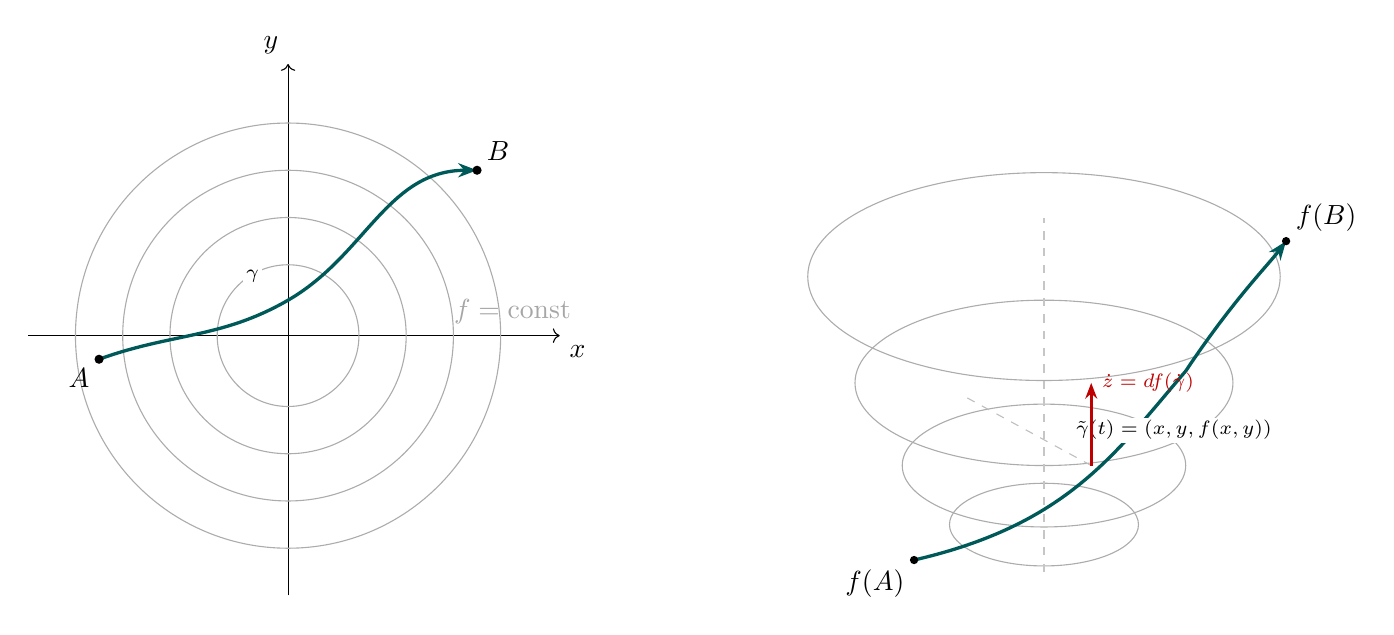
\begin{tikzpicture}[scale=1.5]
	% ========= Left: plane with level sets and path =========
	\begin{scope}[shift={(0,0)}]
		% Axes
		\draw[->] (-2.2,0) -- (2.3,0) node[below right] {$x$};
		\draw[->] (0,-2.2) -- (0,2.3) node[above left] {$y$};
		
		% Level sets (concentric circles)
		\foreach \r in {0.6,1.0,1.4,1.8}{
			\draw[gray!65] (0,0) circle (\r);
		}
		\node[gray!70] at (1.9,0.2) {$f=\text{const}$};
		
		% Path gamma crossing level sets
		\coordinate (A) at (-1.6,-0.2);
		\coordinate (B) at (1.6,1.4);
		\draw[very thick, teal!70!black,
		-{Stealth[length=2.4mm]}]
		(A) to[out=20,in=210] (0.0,0.3) to[out=30,in=180] (B);
		\fill (A) circle (1.1pt) node[below left] {$A$};
		\fill (B) circle (1.1pt) node[above right] {$B$};
		\node[font=\scriptsize, fill=white, inner sep=1pt] at (-0.3,0.5) {$\gamma$};
		
		% A point p on gamma and its gradient (normal)
		\coordinate (p) at (0.2,0.35);
%		\fill (p) circle (1.0pt) node[below right, yshift=-2pt] {$p$};
%		\coordinate (gradTip) at ($(p)!1.0!(0.9,1.05)$);
%		\draw[red!75!black, very thick, -{Stealth[length=2.2mm]}] (p) -- (gradTip)
%		node[above right, xshift=2pt] {$\nabla f(p)$};
		
		% Decompose velocity at p into tangent/normal components
%		\coordinate (tanTip) at ($(p)+( -0.6, 0.2)$);
%		\coordinate (norTip) at ($(p)!0.55!(gradTip)$);
%		\draw[blue!70, very thick, -{Stealth[length=2.2mm]}] (p) -- (tanTip)
%		node[above left, font=\scriptsize] {$\dot\gamma_\parallel$};
%		\draw[orange!80!black, very thick, -{Stealth[length=2.2mm]}] (p) -- (norTip)
%		node[right, font=\scriptsize] {$\dot\gamma_\perp$};
%		\node[font=\scriptsize, fill=white, inner sep=1pt]
%		at (0,-2.15)
%		{$df(\dot\gamma)=\nabla f\!\cdot \dot\gamma
%			=\underbrace{\nabla f\!\cdot \dot\gamma_\parallel}_{0}
%			+\,\nabla f\!\cdot \dot\gamma_\perp$};
	\end{scope}
	
	% ========= Right: 3D-looking lifted curve on z=f(x,y) =========
	\begin{scope}[shift={(6.4,-2)}]
		% Fake-3D axes
%		\draw[->] (-0.2,-0.6) -- (4.2,-0.6) node[right] {$x$};
%		\draw[->] (0,-0.8) -- (0,3.3) node[above] {$z$};
%		\draw[->] (-0.2,-0.6) -- ++(-1.8,1.0) node[left] {$y$};
		
		% Paraboloid wireframe by ellipses (constant z-slices)
		% z = r^2 ; draw ellipses with bigger radii at larger z
		\foreach \z/\rx/\ry in {0.4/0.8/0.35, 0.9/1.2/0.52, 1.6/1.6/0.70, 2.5/2.0/0.88}{
			\draw[gray!65] (0,\z) ellipse [x radius=\rx, y radius=\ry];
		}
		% Central spine (z-axis)
		\draw[gray!45, dashed] (0,0) -- (0,3.0);
		
		% Lift of gamma: a rising curve on the surface
		% We'll sketch by hand with a smooth curve
		\draw[very thick, teal!70!black, -{Stealth[length=2.4mm]}]
		(-1.1,0.1) .. controls (0.2,0.4) and (0.6,1.0) .. (1.2,1.7)
		.. controls (1.6,2.3) and (1.9,2.6) .. (2.05,2.8);
		\node[font=\scriptsize, fill=white, inner sep=1pt] at (1.1,1.2) {$\tilde\gamma(t)=(x,y,f(x,y))$};
		
		% Two corresponding points and vertical speeds
		\coordinate (p2) at (0.4,0.9);
		\draw[gray!50, dashed] (p2) -- ++(-1.1,0.6); % drop to y-axis direction (visual ref)
		\draw[red!75!black, -{Stealth[length=2.0mm]}, very thick] (0.4,0.9) -- +(0,0.7)
		node[right, font=\scriptsize] {$\dot z = df(\dot\gamma)$};
		
		% Endpoints projected
		\fill (-1.1,0.1) circle (1.0pt) node[below left] {$f(A)$};
		\fill (2.05,2.8) circle (1.0pt) node[above right] {$f(B)$};
		
		% Integral = total height change
%		\node[draw, rounded corners, fill=white, align=center, anchor=north west]
%		at (-1.8,3.2)
%		{$\displaystyle \int_\gamma df
%			= \int \dot z\,dt
%			= f(B)-f(A)$};
	\end{scope}
	
\end{tikzpicture}


\begin{tikzpicture}[scale=1.35, >=Stealth]
	
	%==================== LEFT: scalar field + gradient vectors ====================
	\begin{scope}
		% Axes
		\draw[->] (-2.3,0) -- (2.4,0) node[below right] {$x$};
		\draw[->] (0,-2.3) -- (0,2.4) node[above left] {$y$};
		
		% Level sets (circles) of f(x,y)=x^2+y^2
		\foreach \r in {0.7,1.1,1.5,1.9}{
			\draw[gray!65] (0,0) circle (\r);
		}
		\node[gray!60, font=\scriptsize] at (1.95,0.18) {$f=\text{const}$};
		
		% Gradient vectors: ∇f = (2x,2y)
		\def\gscale{0.16}
		\foreach \x in {-2,-1.5,...,2}{
			\foreach \y in {-2,-1.5,...,2}{
				\pgfmathsetmacro{\ux}{2*\x*\gscale}
				\pgfmathsetmacro{\uy}{2*\y*\gscale}
				\draw[gray!30] (\x,\y) circle (0.02);
				\draw[-{Stealth[length=2.0mm]}, line width=0.28pt]
				(\x,\y) -- ++(\ux,\uy);
			}
		}
		
		% Title
		\node[draw, rounded corners, fill=white, align=center, font=\scriptsize]
		at (-1.95,2.1)
		{$f(x,y)=x^2+y^2$\\[1pt]$\nabla f=(2x,2y)$ (vectors)};
	\end{scope}
	
	%==================== RIGHT: covector field df as linelets =====================
	\begin{scope}[xshift=7.0cm]
		% Axes
		\draw[->] (-2.3,0) -- (2.4,0) node[below right] {$x$};
		\draw[->] (0,-2.3) -- (0,2.4) node[above left] {$y$};
		
		% Reference level sets
		\def\R{1.6}
		\draw[gray!55] (0,0) circle (\R);
		\draw[gray!35] (0,0) circle (\R+0.35);
		
		% 1-form glyphs for df = 2x dx + 2y dy:
		% Draw short segments whose normal is (2x,2y) i.e., segments oriented +90° from (x,y).
		\foreach \x in {-2,-1.4,...,2}{
			\foreach \y in {-2,-1.4,...,2}{
				\pgfmathsetmacro{\ang}{atan2(\y,\x) + 90} % linelet direction (deg)
				\pgfmathsetmacro{\r}{sqrt(\x*\x+\y*\y)}
				\pgfmathsetmacro{\len}{0.22 + 0.05*\r}    % mild scaling with |∇f|
				\pgfmathsetmacro{\dx}{0.5*\len*cos(\ang)}
				\pgfmathsetmacro{\dy}{0.5*\len*sin(\ang)}
				\draw[black!70, line width=0.35pt]
				(\x-\dx,\y-\dy) -- (\x+\dx,\y+\dy);
				\fill[black] (\x,\y) circle (0.02);
			}
		}
		
		% At a sample point p: show tangent vs normal action of the covector
		\coordinate (p) at ({\R/sqrt(2)},{\R/sqrt(2)});
		\fill (p) circle (1.1pt) node[above right] {$p$};
		
		% Gradient (normal to linelets)
		\path (0,0) -- (p) coordinate[pos=1.18] (gTip);
		\draw[very thick, red!75!black, -{Stealth[length=2.4mm]}] (p) -- (gTip)
		node[above right, xshift=2pt, font=\scriptsize] {$\nabla f(p)$};
		
		% Tangent direction (parallel to linelets) -> df_p(tangent)=0
		\coordinate (tTip) at ($ (p) + (-0.9,0.9) $);
		\draw[very thick, blue!70, -{Stealth[length=2.2mm]}] (p) -- (tTip)
		node[above left, font=\scriptsize] {$v_{\parallel}$};
		
		% Normal component (across linelets) -> df_p(measures this)
		\coordinate (nTip) at ($ (p)!0.45!(gTip) $);
		\draw[very thick, orange!85!black, -{Stealth[length=2.2mm]}] (p) -- (nTip)
		node[right, font=\scriptsize] {$v_{\perp}$};
		
		% Title
		\node[draw, rounded corners, fill=white, align=center, font=\scriptsize]
		at (-1.95,2.1)
		{$df=2x\,dx+2y\,dy$ (covectors as linelets)\\
			tangent $\to 0$, normal $\to$ measured};
	\end{scope}
	
\end{tikzpicture}

\subsection*{From Gradients to Curl}
Given a vector field $\vec F$, we wish to determine whether $\vec F$ is conservative (i.e., $\vec F=\nabla f$ for some scalar field $f$). Trying to guess the potential function $f$ is hard.

We already know that if a field $\vec{F}$ is conservative, it must be the gradient of some potential function $f$:
\[
\vec{F} = \langle P(x,y), Q(x,y) \rangle = \nabla f = \left\langle \pderiv{f}{x}, \pderiv{f}{y} \right\rangle\tag*{\text{(in 2D)}}
\] What happens if we differentiate $P(x,y) = \pderiv{f}{x}$ with respect to $y$ and $Q(x,y) = \pderiv{f}{y}$ with respect to $x$? \[
\pderiv{P}{y} = \pderiv{}{y}\left(\pderiv{f}{x}\right) = \frac{\partial^2 f}{\partial y \partial x},\quad\quad\pderiv{Q}{x} = \pderiv{}{x}\left(\pderiv{f}{y}\right) = \frac{\partial^2 f}{\partial x \partial y}.
\]
\begin{theorem}[Equality of mixed partials; Clairaut's Theorem]
If the partial derivatives $\spderiv{f}{y}{x}$ and $\spderiv{f}{x}{y}$ exist and are continuous at a point $(a, b)$, then $\spderiv{f}{y}{x}(a,b)=\spderiv{f}{x}{y}(a,b)$, i.e., second order partial derivatives commute if $f$ is $C^2$.
\end{theorem}

%\newpage\noindent
If a vector field $\vec{F} = \langle P(x,y), Q(x,y) \rangle$ is a gradient, it \textbf{must} satisfy the condition \[
\pderiv{Q}{x} = \pderiv{P}{y}.
\]
The quantity $\frac{\partial Q}{\partial x}-\frac{\partial P}{\partial y}$ represents the curl of $\vec F=\langle P,Q\rangle$ and encodes its local rotational behavior. Hence the condition $\frac{\partial Q}{\partial x}=\frac{\partial P}{\partial y}$ (i.e., $\frac{\partial Q}{\partial x}-\frac{\partial P}{\partial y}=0$) means that the field is \textbf{irrotational} (has \textbf{zero curl}).

%\medskip
\newpage
\begin{remark}
Consider a small rectangle centered at \((x_0,y_0)\) with side lengths \(\Delta x,\Delta y\). 
\begin{figure}[h!]
	\centering
	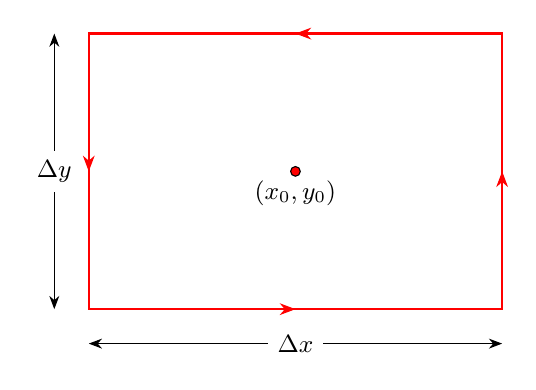
\begin{tikzpicture}[scale=1.75, font=\small, >=Stealth]
		% Draw rectangle and center point
		\draw[thick, red] (-1.5,-1) rectangle (1.5,1);
		\draw[fill=red] (0,0) circle (1pt) node[below] {$(x_0, y_0)$};
		% Add arrows for CCW circulation path
		\draw[-{Stealth[length=2mm]}, red] (-1.5, -1) -- (0, -1);
		\draw[-{Stealth[length=2mm]}, red] (1.5, -1) -- (1.5, 0);
		\draw[-{Stealth[length=2mm]}, red] (1.5, 1) -- (0, 1);
		\draw[-{Stealth[length=2mm]}, red] (-1.5, 1) -- (-1.5, 0);
		\draw[<->] (0-1.5, 0-1.25) -- ++(3, 0) node[midway, fill=white] {$\Delta x$};
		\draw[<->] (0-1.75, 0-1) -- ++(0, 2) node[midway, fill=white] {$\Delta y$};
		% Label path segments
%		\node at (0, -1.7) {Bottom: $\int P(x, y_0-\frac{\Delta y}{2}) dx$};
%		\node at (0, 1.45) {Top: $\int P(x, y_0+\frac{\Delta y}{2}) (-dx)$};
%		\node[rotate=90] at (1.95, 0) {Right: $\int Q(x_0+\frac{\Delta x}{2}, y) dy$};
%		\node[rotate=90] at (-2.2, 0) {Left: $\int Q(x_0-\frac{\Delta x}{2}, y) (-dy)$};
		% Illustrate change in P and Q
%		\draw[->, thick, blue] (0, 1) -- (1.2, 1) node[above] {$P_{top}$};
%		\draw[->, thick, blue] (0, -1) -- (0.8, -1) node[below] {$P_{bot}$};
%		\node[red, align=center] at (2.5, 0) {Difference in P\\contributes\\$-P_y \Delta x \Delta y$};
%		\draw[->, thick, green!50!black] (1.5, 0) -- (1.5, 0.8) node[right] {$Q_{right}$};
%		\draw[->, thick, green!50!black] (-1.5, 0) -- (-1.5, 1.0) node[left] {$Q_{left}$};
%		\node[red, align=center] at (-2.5, 0) {Difference in Q\\contributes\\$Q_x \Delta x \Delta y$};
	\end{tikzpicture}
	\caption{Circulation around an infinitesimal rectangle.}
	\label{fig:local_circ}
\end{figure}

\noindent
The total counterclockwise circulation is the sum of the line integrals along the four edges:
\[
\oint_{\partial R}\vec F\cdot \d\vec r
=\int_{\text{bottom}}P\,\d x+\int_{\text{right}}Q\,\d y+\int_{\text{top}}P\,\d x+\int_{\text{left}}Q\,\d y.
\]
We will approximate the value of $P$ or $Q$ along each edge as being constant, equal to its value at the midpoint of that edge. We find this value using a first-order Taylor expansion from the center point $(x_0, y_0)$.

For a simple function of one variable, $f(x)$, if we know its value at a point $a$, then we can estimate its value at a nearly point $a+h$ using the tangent line at $a$: 
\begin{center}
\begin{minipage}{.49\textwidth}
\begin{align*}
	f(a+h)&\approx f(a)+f'(a)\cdot h \quad\text{or}\\
	f(x)&\approx f(a)+f'(a)\cdot (x-a).
\end{align*} 

\end{minipage}
\begin{minipage}{.49\textwidth}
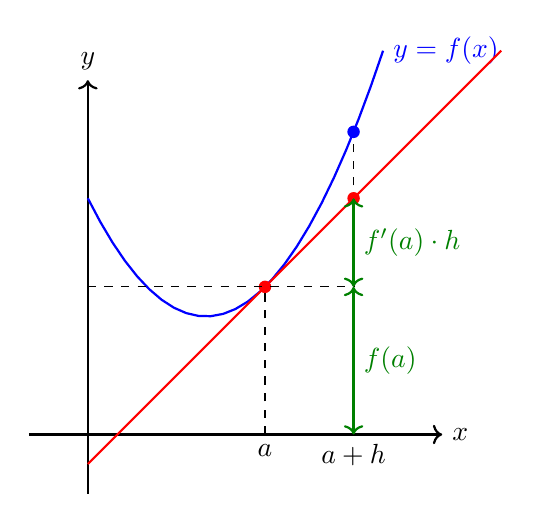
\begin{tikzpicture}[
	scale=1.5,
	declare function={f(\x) = (\x-1)^2 + 1;}
	]
	% Axes
	\draw[->, thick] (-0.5,0) -- (3,0) node[right] {$x$};
	\draw[->, thick] (0,-0.5) -- (0,3) node[above] {$y$};
	% The curve f(x)
	\draw[blue, thick, domain=0:2.5] plot (\x, {f(\x)}) node[right] {$y=f(x)$};
	% Point 'a'
	\def\a{1.5}
	\node[below] at (\a,0) {$a$};
	\draw[dashed] (\a,0) -- (\a, {f(\a)});
	\fill[red] (\a, {f(\a)}) circle (1.5pt);
	% Point 'a+h'
	\def\h{.75}
	\node[below] at (\a+\h,0) {$a+h$};
	\draw[dashed] (\a+\h,0) -- (\a+\h, {f(\a+\h)});
	% Tangent line at 'a'
	% f'(x) = 2(x-1), so f'(a) = 2(a-1)
	\draw[red, thick, domain=0:3.5] plot (\x, {f(\a) + 2*(\a-1)*(\x-\a)});
	% Show f(a)
	\draw[<->, green!50!black, thick] (\a+\h, 0) -- (\a+\h, {f(\a)}) node[midway, right] {$f(a)$};
	% Show the approximation f(a) + f'(a)h
	\pgfmathsetmacro{\approxY}{f(\a) + 2*(\a-1)*\h}
	\fill[red] (\a+\h, \approxY) circle (1.5pt);
%	\draw[red, dashed] (\a+\h, \approxY) -- (\a+\h, 0);
	
	% Show the actual value f(a+h)
	\fill[blue] (\a+\h, {f(\a+\h)}) circle (1.5pt);
%	\node[right, blue] at (\a+\h, {f(\a+\h)}) {Actual value: $f(a+h)$};
%	\node[right, red] at (\a+\h, \approxY) {Approximation: $f(a)+f'(a)h$};
	
	% Label the components of the approximation
	\draw[<->, green!50!black, thick] (\a+\h, {f(\a)}) -- (\a+\h, \approxY) node[midway, right] {$f'(a)\cdot h$};
	\draw[dashed] (0, {f(\a)}) -- (\a+\h, {f(\a)});
\end{tikzpicture}
\end{minipage}
\end{center}
In words, ``New Value $\approx$ Old Value + (Rate of Change) $\times$ (Small Step)''. 

\newpage\noindent
For a function of two variables like $P(x,y)$, the idea is identical, but the ``rate of change'' now has two components (one for each direction), and the ``tangent line'' becomes a ``tangent plane''.
The general first-order Taylor expansion for $P(x,y)$ around a center point $(x_0,y_0)$ is
\[
P(x_0+a, y_0+b) \approx P(x_0, y_0) + \pderiv{P}{x}(x_0, y_0) \cdot a + \pderiv{P}{y}(x_0, y_0) \cdot b
\] Here, $a$ is the small step in the $x$-direction, and $b$ is the small step in the $y$-direction.

\paragraph{1. The Horizontal Paths}
These integrals involve the horizontal component of $P(x,y)$.
\begin{itemize}
	\item \textbf{Bottom Path ($\rightarrow$):} 
	\[ P\left(x, y_0 - \frac{\Delta y}{2}\right) \approx P(x_0,y_0) - \pderiv{P}{y}\frac{\Delta y}{2}\implies
	\int_{\text{bottom}} P\,\d x \approx \left( P(x_0,y_0) - \pderiv{P}{y}\frac{\Delta y}{2} \right) (\Delta x) \]
	\item \textbf{Top Path ($\leftarrow$):}
	\[ P\left(x, y_0 + \frac{\Delta y}{2}\right) \approx P(x_0,y_0) + \pderiv{P}{y}\frac{\Delta y}{2}\implies\int_{\text{top}}P\,\d x \approx -\left( P(x_0,y_0) + \pderiv{P}{y}\frac{\Delta y}{2} \right) (\Delta x) \]
\end{itemize} Here, we are left with only the parts that describe the \textit{change} in $P$ with respect to $y$.
\[
\int_{\text{bottom}} P\,\d x + \int_{\text{top}} P\,\d x \approx \left(-\pderiv{P}{y}\frac{\Delta y}{2}\right)\Delta x - \left(\pderiv{P}{y}\frac{\Delta y}{2}\right)\Delta x = -\pderiv{P}{y}\Delta x\Delta y
\]
\paragraph{2. The Vertical Paths}
These integrals involve the vertical component of $Q(x,y)$.
\begin{itemize}
	\item \textbf{Right Path ( $\uparrow$ ):} 
	\[ Q\left(x_0 + \frac{\Delta x}{2}, y\right) \approx Q(x_0,y_0) + \pderiv{Q}{x}\frac{\Delta x}{2}\implies\int_{\text{right}}Q\,\d y \approx \left( Q(x_0,y_0) + \pderiv{Q}{x}\frac{\Delta x}{2} \right) (\Delta y) \]
	\item \textbf{Left Path ( $\downarrow$ ):} 
	\[ Q\left(x_0 - \frac{\Delta x}{2}, y\right) \approx Q(x_0,y_0) - \pderiv{Q}{x}\frac{\Delta x}{2}\implies\int_{\text{left}}Q\,\d y \approx -\left( Q(x_0,y_0) - \pderiv{Q}{x}\frac{\Delta x}{2} \right) (\Delta y) \]
\end{itemize} Here, we are left with only the parts that describe the \textit{change} in $Q$ with respect to $x$.
\[
\int_{\text{right}}Q\,\d y + \int_{\text{left}}Q\,\d y \approx \left(\pderiv{Q}{x}\frac{\Delta x}{2}\right)\Delta y + \left(\pderiv{Q}{x}\frac{\Delta x}{2}\right)\Delta y = \pderiv{Q}{x}\Delta x\Delta y
\]

Now we sum the results from the horizontal and vertical pairs:
\begin{align*}
	\oint_{\partial R}\vec F\cdot d\vec r &\approx \left(-\pderiv{P}{y}\Delta x\Delta y\right) + \left(\pderiv{Q}{x}\Delta x\Delta y\right) \\
	&= \left(\pderiv{Q}{x} - \pderiv{P}{y}\right)\Delta x\Delta y
\end{align*}
This shows that the total circulation around the tiny loop is approximately the quantity $\left(\pderiv{Q}{x} - \pderiv{P}{y}\right)$ multiplied by the area of the loop ($\Delta A = \Delta x \Delta y$).

To get the property \textit{at the point} $(x_0, y_0)$, we find the circulation \textbf{density}. We divide by the area and take the limit as the rectangle shrinks to zero.
\[
\lim_{\Delta A\to 0}\frac{1}{\Delta A}\oint_{\partial R}\vec F\cdot \d\vec r = \pderiv{Q}{x}(x_0, y_0) - \pderiv{P}{y}(x_0, y_0)
\]
This is why we call the scalar quantity $\pderiv{Q}{x} - \pderiv{P}{y}$ the \textbf{curl}: it is the circulation per unit area at a point, which measures the local rotational tendency of the field.

\end{remark}

\begin{remark}
If \(C=\partial D\) is a positively oriented simple closed curve enclosing a region \(D\),
Green's theorem states \[
%\oint_{C}\vec F\cdot\d\vec r
%=\iint_{D}\Big(\frac{\partial Q}{\partial x}-\frac{\partial P}{\partial y}\Big)\,\d A.
\underbrace{\oint_{C}\vec F\cdot\d\vec r}_{\substack{\textbf{Line Integral}\\ \textbf{(Total Circulation)}}}= \underbrace{\iint_{D}\Big(\frac{\partial Q}{\partial x}-\frac{\partial P}{\partial y}\Big)\,\d A}_{\substack{\textbf{Double Integral}\\ \textbf{(Sum of Local Curls)}}}
\]
%So the total circulation equals the area integral of the local circulation density.
\begin{center}
\begin{tikzpicture}[scale=1.5, >=Stealth]
	% Style for the main curve and region
	\tikzstyle{maincurve}=[thick, blue, postaction={decorate, decoration={markings, mark=at position 0.1 with {\arrow{>}}, mark=at position 0.35 with {\arrow{>}}, mark=at position 0.6 with {\arrow{>}}, mark=at position 0.85 with {\arrow{>}}}}]
	\tikzstyle{mainregion}=[thick, blue, fill=blue!10]
	% 1. Draw the main region D and its boundary C
	\draw[mainregion] plot [smooth cycle, tension=0.7] coordinates {(0,0) (5,1) (6,4) (3,5) (-1,3)};
	\node[blue] at (6.75, 1.5) {\Large $C = \partial D$};
	\draw[maincurve] plot [smooth cycle, tension=0.7] coordinates {(0,0) (5,1) (6,4) (3,5) (-1,3)};
	% Clip the grid to the shape of D
	\begin{scope}
		\clip plot [smooth cycle, tension=.7] coordinates {(0,0) (5,1) (6,4) (3,5) (-1,3)};
		% Draw a faint grid representing dA elements
%		\draw[gray!50, thin, step=1] (-2,-1) grid (8,5);
		\def\step{0.70} % Match the grid step size
		% Loop to draw multiple rectangles
		% x_coord from 0 to 5, y_coord from 1 to 4 (adjust these ranges to cover your desired area)
		\foreach \xcoord in {-2,-1.25, ..., 6} { % Start, step, end for x
			\foreach \ycoord in {-.75, 0, ..., 4.5} { % Start, step, end for y
				\draw[fill=red] (\xcoord+\step/2,\ycoord+\step/2) circle (2pt);
				% Draw the four edges of each rectangle with the arrow style
				\draw[red, thin, ->] (\xcoord,\ycoord) -- (\xcoord+\step/2,\ycoord);
				\draw[red, thin, -] (\xcoord+\step/2,\ycoord) -- (\xcoord+\step,\ycoord);
				\draw[red, thin, ->] (\xcoord+\step,\ycoord) -- (\xcoord+\step,\ycoord+\step/2);
				\draw[red, thin, -] (\xcoord+\step,\ycoord+\step/2) -- (\xcoord+\step,\ycoord+\step);
				\draw[red, thin, ->] (\xcoord+\step,\ycoord+\step) -- (\xcoord+\step/2,\ycoord+\step);
				\draw[red, thin, -] (\xcoord+\step/2,\ycoord+\step) -- (\xcoord,\ycoord+\step);
				\draw[red, thin, ->] (\xcoord,\ycoord+\step) -- (\xcoord,\ycoord+\step/2);
				\draw[red, thin, ->] (\xcoord,\ycoord+\step/2) -- (\xcoord,\ycoord);
			}
		}
	\end{scope}
\end{tikzpicture}
\end{center}
\end{remark}



\section*{Example 1: Rigid rotation and angular velocity}
Consider the rigid rotation field with angular speed \(\omega\):
\[
\vec F(x,y)=\langle -\omega y,\ \omega x\rangle.
\]
Then
\[
\frac{\partial Q}{\partial x}=\omega,\qquad \frac{\partial P}{\partial y}=-\omega
\quad\Rightarrow\quad
\operatorname{curl}\vec F = Q_x - P_y = 2\omega.
\]
This shows curl equals twice the angular velocity. For a circle of radius \(R\),
parametrize \(r(t)=(R\cos t,R\sin t)\), \(dr=(-R\sin t,R\cos t)\,dt\). Then
\[
\oint \vec F\cdot d\vec r
=\int_0^{2\pi}\omega R^2\,dt
=2\pi\omega R^2.
\]
Meanwhile, \(\iint_{D}(2\omega)\,dA=2\omega \cdot \pi R^2=2\pi\omega R^2\), agreeing with Green's theorem.

\section*{Example 2: Curl-free but not conservative (topology matters)}
On \(\mathbb{R}^2\setminus\{(0,0)\}\), define
\[
\vec F(x,y)=\Big\langle -\frac{y}{x^2+y^2},\ \frac{x}{x^2+y^2}\Big\rangle.
\]
A direct calculation shows \(Q_x-P_y=0\) wherever defined (curl-free). However, the circulation
around the unit circle is
\[
\oint \vec F\cdot d\vec r=2\pi\neq 0.
\]
Hence there is no global potential function; the puncture creates a topological obstruction.
This illustrates that \(\operatorname{curl}\vec F=0\) captures \emph{local} rotation, while global
circulation can persist in domains with holes.

\section*{Summary checklist}
\begin{itemize}
	\item \(Q_x-P_y\) is the infinitesimal (per-area) circulation density.
	\item Green's theorem sums local curl to give total circulation.
	\item Rigid rotation: \(\operatorname{curl}=2\omega\) (twice angular velocity).
	\item Curl \(=0\) can still have nonzero loop integrals if the domain has holes.
\end{itemize}

\newpage
\subsection*{Test 1: Equality of Mixed Partials}
\subsection*{Test 2: Path Independence}
\subsection*{Test 3: Potential Recovery}

%\begin{example}
%Consider the simple vector field $\vec F(x,y) = \langle y, 0 \rangle$.
%
%\begin{center}
%\begin{tikzpicture}
%	\begin{axis}
%		[
%		axis lines = middle,
%		xmin = -3, xmax = 3,
%		ymin = -3, ymax = 3,
%		zmin = 0, zmax = 1,
%		axis equal image,
%		view = {0}{90},
%		]
%		\addplot3
%		[
%		quiver =
%		{
%			u = {y},
%			v = {0},
%		},
%		-stealth,
%		domain = -2:2,
%		domain y = -2:2,
%		red
%		] {0};
%	\end{axis}
%\end{tikzpicture}
%\end{center}
%\end{example}
%
%\begin{tikzpicture}[
%	scale=1.5,
%	font=\Large,
%	% Define styles for different elements
%	vector/.style={-stealth, blue, thick},
%	point/.style={circle, fill, inner sep=1.5pt},
%	label/.style={font=\large},
%	calc/.style={font=\huge, align=left}
%	]
%	% --- Visualization for dP/dy ---
%	\node[label, align=center] at (0, 3) {Horizontal Component ($P=y$)\\changes with $y$};
%	% Draw two points vertically aligned
%	\node[point, label={[label]right: $(x, y)$}] (p1) at (0, 1) {};
%	\node[point, label={[label]right: $(x, y+\Delta y)$}] (p2) at (0, 2) {};
%	% Draw vectors at these points, F=<y,0>
%	\draw[vector] (p1) -- ++(1, 0) node[anchor=west]{$\vv{F}(x,y) = \langle y, 0 \rangle$};
%	\draw[vector] (p2) -- ++(2, 0) node[anchor=west]{$\vv{F}(x,y+\Delta y) = \langle y+\Delta y, 0 \rangle$};
%	% Dashed line to show vertical change
%	\draw[dashed, thick] (p1) -- (p2);
%	\node[calc, green!50!black] at (1.5, 0) {$\pdv{P}{y} = \pdv{}{y}(y) = 1$};
%	
%	% --- Visualization for dQ/dx ---
%	\node[label, align=center] at (5, 3) {Vertical Component ($Q=0$)\\does not change with $x$};
%	% Draw two points horizontally aligned
%	\node[point, label={[label]right: $(x, y)$}] (q1) at (5, 1.5) {};
%	\node[point, label={[label]right: $(x+\Delta x, y)$}] (q2) at (6.5, 1.5) {};
%	% Note that the vertical component is 0 at both points
%	\node[label, gray] at (q1) [below=5pt] {Vertical component $Q=0$};
%	\node[label, gray] at (q2) [below=5pt] {Vertical component $Q=0$};
%	% Dashed line to show horizontal change
%	\draw[dashed, thick] (q1) -- (q2);
%	\node[calc, red] at (6, 0) {$\pdv{Q}{x} = \pdv{}{x}(0) = 0$};
%	
%	% --- Divider Line ---
%	\draw[gray, very thick] (3.5, -1) -- (3.5, 3.5);
%	
%	% --- Final Curl Calculation ---
%	\node[calc, align=center] at (3.5, -2) {
%		Curl = $\underbrace{\pdv{Q}{x}}_{\color{red}0} - \underbrace{\pdv{P}{y}}_{\color{green!50!black}1} = 0 - 1 = -1$
%	};
%\end{tikzpicture}

\newpage
\section{Del to Differential ($\nabla\to\d$)}
\subsection{What is a covector?}
\begin{observation}
For $\alpha=\begin{bmatrix}2 & 1\end{bmatrix}\in(\R^2)^*$ and any $\vec{v}=\begin{bmatrix}
x \\ y \end{bmatrix}\in \R^2$, \[
\alpha(\vec{v})=\begin{bmatrix}
	2 & 1 \end{bmatrix}\begin{bmatrix}
	x \\ y \end{bmatrix}=(2)(x)+(1)(y)=2x+y.
\] 
%\textbf{Geometric read:} thinking of the parallel lines $2x+y=c$, vectors that slide \emph{along} a line add no contribution; only the component \emph{across} lines contributes, and contributions add (superpose) because the pairing is linear.
\end{observation}
\begin{definition}
Let $V=\mathbb{R}^n$. A \emph{covector} (or \emph{linear functional}) is a linear map \[
\alpha:V\to \R,\qquad\vec{v}\mapsto\alpha(\vec{v})=\begin{bmatrix}
		\alpha_1 & \cdots & \alpha_n
	\end{bmatrix}\begin{bmatrix}
	v^1\\ \vdots \\ v^n
\end{bmatrix}=\sum_{i=0}^n\alpha_iv^i.
%\qquad\text{such that}\qquad \alpha(a\vec{v}_1+b\vec{v}_2)=a\,\alpha(\vec{v}_1)+b\,\alpha(\vec{v}_2).
\]
The set of all covectors is the dual space $V^*=\mathrm{Hom}(V,\mathbb{R})$.
\end{definition}
\vfill
\begin{remark}
For covectors $\alpha,\beta\in V^*$ and $c\in\mathbb R$,
\[
(\alpha+\beta)(\vec{v})=\alpha(\vec{v})+\beta(\vec{v}),\qquad
(c\alpha)(\vec{v})=c\alpha(\vec{v})\quad \text{for all } \vec{v}\in V.
\]
So $V^*$ is a vector space with these operations.
\end{remark}
\vfill
\begin{observation}[Level sets]
	The value of $\alpha$ is constant on the \emph{level sets}
	\[
	2x+y=c,\qquad c\in\mathbb{R}.
	\]
\begin{center}
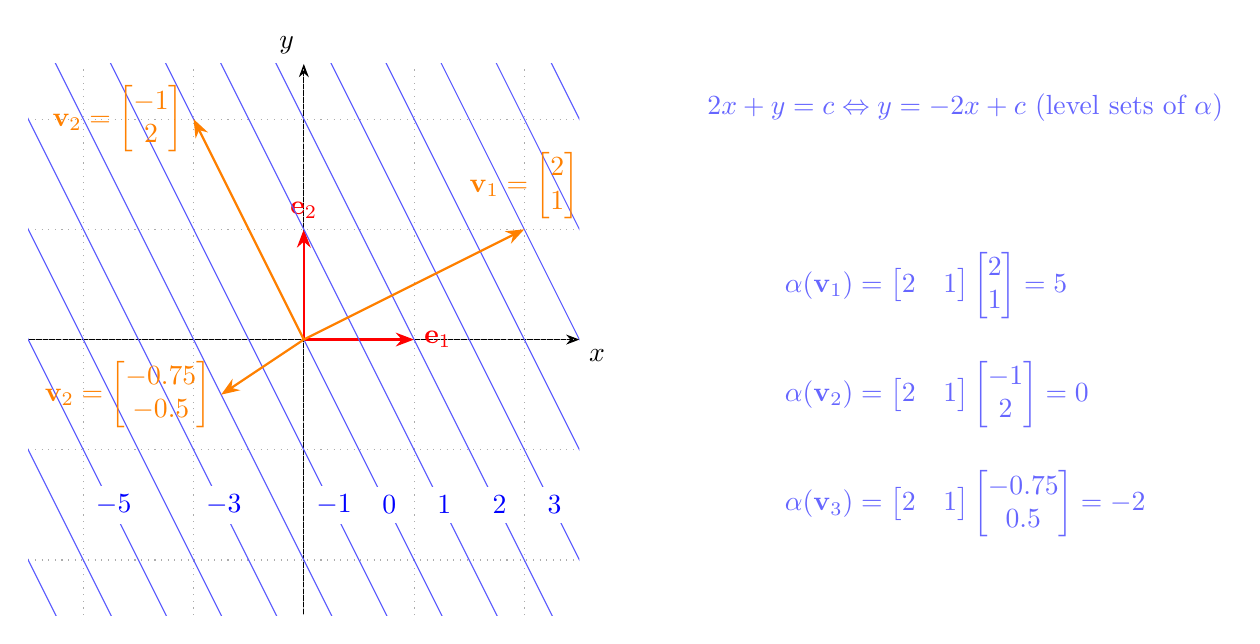
\begin{tikzpicture}[scale=1.4, >=Stealth]
	% Axes
	\draw[->] (-2.5,0) -- (2.5,0) node[below right] {$x$};
	\draw[->] (0,-2.5) -- (0,2.5) node[above left] {$y$};
	% Parallel level sets: 2x + y = c  (c from -3 to 3)
	\begin{scope}
		\clip (-2.5,-2.5) rectangle (2.5,2.5); % (xmin,ymin) rectangle (xmax,ymax)
		\draw[dotted, gray!65] (-2.5,-2.5) grid (2.5,2.5);
		\draw[->, thick, red] (0,0) -- ++(1,0) node[right] {$\vec{e}_1$};
		\draw[->, thick, red] (0,0) -- ++(0,1) node[above] {$\vec{e}_2$};
		% Parallel level sets: 2x + y = c  (c from -3 to 3)
		\foreach \c in {-7,-6,...,7}{
			\draw[blue!65] plot[domain=-10:10] (\x, {\c - 2*\x});
			
		}
		\foreach \x in {-1,...,3}{
			\node[fill=white] at (.775+0.5*\x,-1.5) {\color{blue}$\x$};
		}
		\foreach \x in {-5,-3}{
			\node[fill=white] at (.775+0.5*\x,-1.5) {\color{blue}$\x$};
		}
		\draw[->, thick, orange] (0,0) -- ++(2,1) node[above] {$\vec{v}_1=\begin{bmatrix}
			2\\ 1
		\end{bmatrix}$};
		\draw[->, thick, orange] (0,0) -- ++(-1,2) node[left] {$\vec{v}_2=\begin{bmatrix}
			-1\\ 2
		\end{bmatrix}$};
		\draw[->, thick, orange] (0,0) -- ++(-0.75,-.5) node[left] {$\vec{v}_2=\begin{bmatrix}
			-0.75\\ -0.5
		\end{bmatrix}$};
	\end{scope}
	\node[blue!60] at (6,2.1) {$2x+y=c\Leftrightarrow y=-2x+c$ (level sets of $\alpha$)};
	\node[blue!60, align=left] at (6,-.5) {$\alpha(\vec{v}_1)=\begin{bmatrix}
			2 & 1
		\end{bmatrix}\begin{bmatrix}
		2 \\  1
	\end{bmatrix}=5$\\ \\ \\
	$\alpha(\vec{v}_2)=\begin{bmatrix}
		2 & 1
	\end{bmatrix}\begin{bmatrix}
		-1 \\  2
	\end{bmatrix}=0$\\ \\ \\
	$\alpha(\vec{v}_3)=\begin{bmatrix}
		2 & 1
	\end{bmatrix}\begin{bmatrix}
		-0.75 \\  0.5
	\end{bmatrix}=-2$};
\end{tikzpicture}
\end{center}

\newpage
\begin{center}
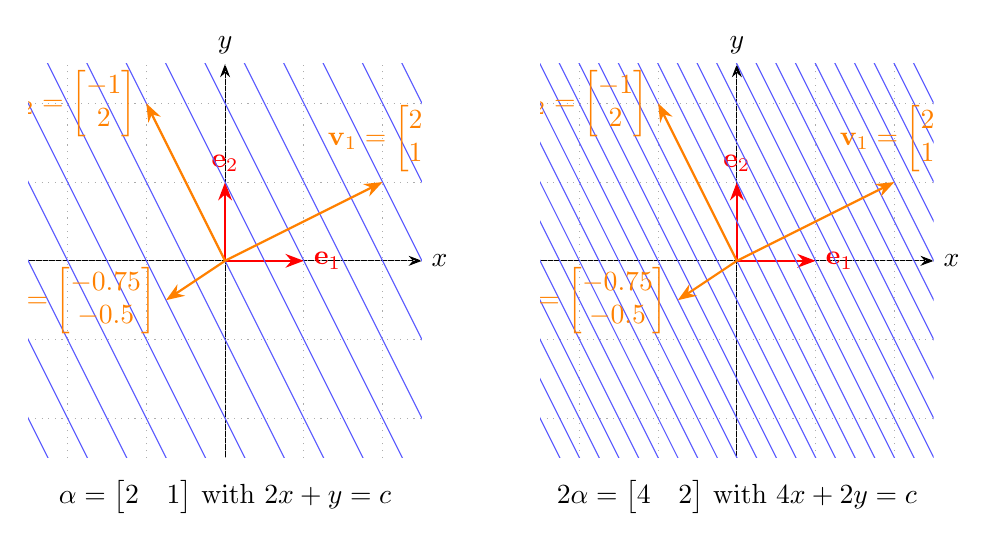
\begin{tikzpicture}[scale=1, >=Stealth]
	\draw[->] (-2.5,0) -- (2.5,0) node[right] {$x$};
	\draw[->] (0,-2.5) -- (0,2.5) node[above] {$y$};
	% Parallel level sets: 2x + y = c  (c from -3 to 3)
	\begin{scope}
		\clip (-2.5,-2.5) rectangle (2.5,2.5); % (xmin,ymin) rectangle (xmax,ymax)
		\draw[dotted, gray!65] (-2.5,-2.5) grid (2.5,2.5);
		\draw[->, thick, red] (0,0) -- ++(1,0) node[right] {$\vec{e}_1$};
		\draw[->, thick, red] (0,0) -- ++(0,1) node[above] {$\vec{e}_2$};
		% Parallel level sets: 2x + y = c  (c from -3 to 3)
		\foreach \c in {-7,-6,...,7}{
			\draw[blue!65] plot[domain=-10:10] (\x, {\c - 2*\x});
		}
		\draw[->, thick, orange] (0,0) -- ++(2,1) node[above] {$\vec{v}_1=\begin{bmatrix}
				2\\ 1
			\end{bmatrix}$};
		\draw[->, thick, orange] (0,0) -- ++(-1,2) node[left] {$\vec{v}_2=\begin{bmatrix}
				-1\\ 2
			\end{bmatrix}$};
		\draw[->, thick, orange] (0,0) -- ++(-0.75,-.5) node[left] {$\vec{v}_2=\begin{bmatrix}
				-0.75\\ -0.5
			\end{bmatrix}$};
	\end{scope}
	\node at (0,-3) {$\alpha=\begin{bmatrix}
			2 & 1
		\end{bmatrix}$ with $2x+y=c$};
	\draw[->] (6.5+-2.5,0) -- (6.5+2.5,0) node[right] {$x$};
	\draw[->] (6.5+0,-2.5) -- (6.5+0,2.5) node[above] {$y$};
	\begin{scope}[xshift=6.5cm]
		\clip (-2.5,-2.5) rectangle (2.5,2.5); % (xmin,ymin) rectangle (xmax,ymax)
		\draw[dotted, gray!65] (-2.5,-2.5) grid (2.5,2.5);
		\draw[->, thick, red] (0,0) -- ++(1,0) node[right] {$\vec{e}_1$};
		\draw[->, thick, red] (0,0) -- ++(0,1) node[above] {$\vec{e}_2$};
		% Parallel level sets: 2x + y = c  (c from -3 to 3)
		\foreach \c in {-14,-13,...,14}{
			\draw[blue!65] plot[domain=-10:10] (\x, {\c*.5 - 2*\x});	
		}
		\draw[->, thick, orange] (0,0) -- ++(2,1) node[above] {$\vec{v}_1=\begin{bmatrix}
				2\\ 1
			\end{bmatrix}$};
		\draw[->, thick, orange] (0,0) -- ++(-1,2) node[left] {$\vec{v}_2=\begin{bmatrix}
				-1\\ 2
			\end{bmatrix}$};
		\draw[->, thick, orange] (0,0) -- ++(-0.75,-.5) node[left] {$\vec{v}_2=\begin{bmatrix}
				-0.75\\ -0.5
			\end{bmatrix}$};
	\end{scope}
	\node at (6.5,-3) {$2\alpha=\begin{bmatrix}
		4 & 2
	\end{bmatrix}$ with $4x+2y=c$};
\end{tikzpicture}
\end{center}
\vfill
\begin{center}
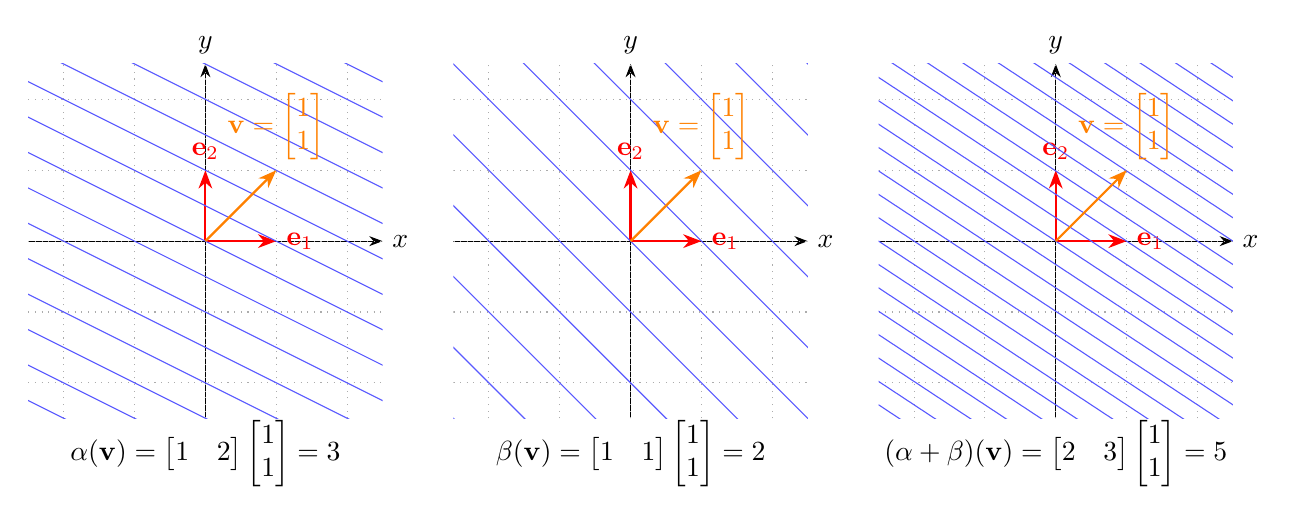
\begin{tikzpicture}[scale=.9, >=Stealth]
	\draw[->] (-2.5,0) -- (2.5,0) node[right] {$x$};
	\draw[->] (0,-2.5) -- (0,2.5) node[above] {$y$};
	% Parallel level sets: 2x + y = c  (c from -3 to 3)
	\begin{scope}
		\clip (-2.5,-2.5) rectangle (2.5,2.5); % (xmin,ymin) rectangle (xmax,ymax)
		\draw[dotted, gray!65] (-2.5,-2.5) grid (2.5,2.5);
		\draw[->, thick, red] (0,0) -- ++(1,0) node[right] {$\vec{e}_1$};
		\draw[->, thick, red] (0,0) -- ++(0,1) node[above] {$\vec{e}_2$};
		% Parallel level sets: 2x + y = c  (c from -3 to 3)
		\foreach \c in {-14,-13,...,14}{
			\draw[blue!65] plot[domain=-10:10] (\x, {\c*.5 - .5*\x});
		}
		\draw[->, thick, orange] (0,0) -- ++(1,1) node[above] {$\vec{v}=\begin{bmatrix}
			1\\ 1
		\end{bmatrix}$};
	\end{scope}
	\node at (0,-3) {$\alpha(\vec{v})=\begin{bmatrix}
		1 & 2
	\end{bmatrix}\begin{bmatrix}
		1 \\ 1
	\end{bmatrix}=3$};
	
	\draw[->] (6+-2.5,0) -- (6+2.5,0) node[right] {$x$};
	\draw[->] (6+0,-2.5) -- (6+0,2.5) node[above] {$y$};
	\begin{scope}[xshift=6cm]
		\clip (-2.5,-2.5) rectangle (2.5,2.5); % (xmin,ymin) rectangle (xmax,ymax)
		\draw[dotted, gray!65] (-2.5,-2.5) grid (2.5,2.5);
		\draw[->, thick, red] (0,0) -- ++(1,0) node[right] {$\vec{e}_1$};
		\draw[->, thick, red] (0,0) -- ++(0,1) node[above] {$\vec{e}_2$};
		% Parallel level sets: 2x + y = c  (c from -3 to 3)
		\foreach \c in {-20,-19,...,20}{
			\draw[blue!65] plot[domain=-10:10] (\x, {\c - \x});
			
		}
		\draw[->, thick, orange] (0,0) -- ++(1,1) node[above] {$\vec{v}=\begin{bmatrix}
				1\\ 1
		\end{bmatrix}$};
	\end{scope}
	\node at (6,-3) {$\beta(\vec{v})=\begin{bmatrix}
			1 & 1
		\end{bmatrix}\begin{bmatrix}
			1 \\ 1
		\end{bmatrix}=2$};
	
	\draw[->] (12+-2.5,0) -- (12+2.5,0) node[right] {$x$};
	\draw[->] (12+0,-2.5) -- (12+0,2.5) node[above] {$y$};
	\begin{scope}[xshift=12cm]
		\clip (-2.5,-2.5) rectangle (2.5,2.5); % (xmin,ymin) rectangle (xmax,ymax)
		\draw[dotted, gray!65] (-2.5,-2.5) grid (2.5,2.5);
		\draw[->, thick, red] (0,0) -- ++(1,0) node[right] {$\vec{e}_1$};
		\draw[->, thick, red] (0,0) -- ++(0,1) node[above] {$\vec{e}_2$};
		% Parallel level sets: 2x + y = c  (c from -3 to 3)
		\foreach \c in {-14,-13,...,14}{
			\draw[blue!65] plot[domain=-10:10] (\x, {\c*.33 - .66*\x});
		}
		\draw[->, thick, orange] (0,0) -- ++(1,1) node[above] {$\vec{v}=\begin{bmatrix}
			1\\ 1
		\end{bmatrix}$};
	\end{scope}
	\node at (12,-3) {$(\alpha+\beta)(\vec{v})=\begin{bmatrix}
			2 & 3
		\end{bmatrix}\begin{bmatrix}
			1 \\ 1
		\end{bmatrix}=5$};
\end{tikzpicture}
\end{center}
\vfill
%\begin{note}[Linearity of differentials]
%If $f,g:\mathbb R^n\to\mathbb R$ are smooth and $c\in\mathbb R$, 
%\[
%\d(f+g)=\d f+\d g,\qquad \d(cf)=c\d f,
%\]
%so differentials $\d f$ are covector fields.
%\end{note}
%Each is a straight line with Euclidean normal vector $(2,1)$. Moving \emph{along} one of these lines does not change the value of $\alpha$; moving \emph{across} them (in the direction of the normal) changes $\alpha$ most quickly.
\begin{center}
\begin{tikzpicture}
	\draw[-Stealth] (7,4) -- ++ (1,0) node[midway, above] {$\nabla=\left(\pderiv{}{x}, \pderiv{}{y}\right)$};
	\begin{groupplot}[
		group style={group size=2 by 1, horizontal sep=2.2cm},
		width=9cm, height=8cm,
		xmin=-2, xmax=2, ymin=-2, ymax=2,
		domain=-2:2, y domain=-2:2,
%		colormap/viridis,
		axis on top,
		]
		% --- Panel 1: Heatmap of f with gradient field arrows (top-down view) ---
		\nextgroupplot[
		title={Scalar field $f(x,y)=2x+y$},
		view={0}{90},
		axis equal image,
		xlabel={$x$}, ylabel={$y$},
		ticks=none,
		]
		% Heatmap (top-down view of the surface)
		\addplot3[
		surf, shader=interp,
		samples=45, samples y=45,
		colormap/cool
		] {2*x + y};
		
		% --- Panel 2: 3D surface z = f(x,y) ---
		\nextgroupplot[
		title={Gradient field $\nabla f=\langle 2,1\rangle$},
		view={0}{90},
		axis equal image,
		xlabel={$x$}, ylabel={$y$},
		ticks=none,
		]		
		% Gradient field arrows: (2x, 2y)
		\addplot3[
		-stealth,
		quiver={
			u=2, v=1, w=0,
			scale arrows=0.12
		},
		samples=16,
		samples y=16,
		domain=-2:1.8, y domain=-2:1.8,
		] ({x},{y},{0});
	\end{groupplot}
\end{tikzpicture}
\end{center}

%\begin{tikzpicture}
%\begin{groupplot}[
%	group style={group size=2 by 1, horizontal sep=1.8cm},
%	width=9cm, height=8cm,
%	xmin=-2, xmax=2, ymin=-2, ymax=2,
%	domain=-2:2, y domain=-2:2,
%	colormap/viridis,
%	axis on top,
%	]
%	% --- Panel 1: Heatmap of f with gradient field arrows (top-down view) ---
%	\nextgroupplot[
%	title={Scalar field $f(x,y)=2x+y$ with $\nabla f$},
%	view={0}{90},
%	axis equal image,
%	xlabel={$x$}, ylabel={$y$},
%	ticks=none,
%	colormap/cool
%	]
%	\addplot3[
%	surf, shader=interp,
%	samples=45, samples y=45,
%	] {2*x + y};
%	\addplot3[
%	-stealth,
%	quiver={
%		u=2, v=1, w=0,
%		scale arrows=0.12
%	},
%	samples=16,
%	samples y=16,
%	domain=-2:1.8, y domain=-2:1.8,
%	] ({x},{y},{0});
%	% --- Panel 2: 3D surface z = f(x,y) ---
%	\nextgroupplot[
%%	axis lines = middle,
%	title={$z=f(x,y)=x^2+y^2$ (surface)},
%%	view={125}{25},
%	view={0}{90},
%	axis equal image,
%	xlabel={$x$}, ylabel={$y$}, zlabel={$z$},
%	samples=50, samples y=50,
%%	zmin=0,
%	ticks=none,
%	colormap/cool
%	]
%	\addplot3[
%	surf, shader=interp
%	] {2*x+y};
%	\addplot3[
%		samples=16,	samples y=16,
%		domain=-2:1.8, y domain=-2:1.8,
%		red
%	] {2*x+y};
%\end{groupplot}
%\end{tikzpicture}
\end{observation}

\newpage
%\paragraph{Kernel (tangent directions).}
%The kernel of $\alpha$ is
%\[
%\ker\alpha=\{v\in\mathbb{R}^2:\alpha(v)=0\}
%=\{(x,y):2x+y=0\}
%=\{\,(-t,2t):t\in\mathbb{R}\,\}.
%\]
%These are precisely the \emph{tangent} directions to the level lines; $\alpha$ \emph{kills} them: $\alpha(v_{\parallel})=0$.
%
%\paragraph{Normal directions.}
%A normal vector is any nonzero multiple of $(2,1)$. For $v_{\perp}=\lambda(2,1)$ we have
%$\alpha(v_{\perp})=2(2\lambda)+1(\lambda)=5\lambda$ (nonzero unless $\lambda=0$). Thus $\alpha$ measures only the \emph{across-level} component of motion.
%\section*{3. Relation to angle/projection}
%If $u$ is a unit vector making angle $\phi$ with the normal $(2,1)$, then
%\[
%\alpha(u)=\|\alpha\|\,\|u\|\cos\phi = \|\alpha\|\cos\phi,
%\]
%where in the Euclidean identification $V\simeq V^*$ we read $\alpha$ as the vector $(2,1)$ and $\|\alpha\|=\sqrt{2^2+1^2}=\sqrt{5}$. This shows $\alpha$ is the (scaled) orthogonal projection onto its normal direction.
%
%\section*{4. Quick numeric check}
%At $v_{\parallel}=(-1,2)$ (tangent), $\alpha(v_{\parallel})=2(-1)+1(2)=0$. \\
%At $v_{\perp}=(2,1)$ (normal), $\alpha(v_{\perp})=2(2)+1(1)=5$.


\newpage
\subsection{Dual basis}
Let $V$ be a $\R$-vector space with basis $\{\vec{e}_1,\vec{e}_2\}$. A \emph{covector} is a linear functional
\[
\alpha:V\to\R,\qquad \alpha(a\vec{v}_1+b\vec{v}_2)=a\,\alpha(\vec{v}_1)+b\,\alpha(\vec{v}_2).
\]
The collection of all covectors is the \emph{dual space} \(V^*=\mathrm{Hom}(V,\R)\).

We cannot use a basis of $V$ to measure covectors directly. To measure covectors, we use the
dual basis of \(V^*\).  Given a basis \(\{\vec{e}_1,\vec{e}_2\}\) of \(V\), the \emph{dual basis} \(\{\varepsilon^1,\varepsilon^2\}\subset V^*\) is defined by \[
\varepsilon^{i}(\vec{e}_j)=\delta_{ij}=\begin{cases}
	1 &:i=j\\
	0 &:i\neq j
\end{cases}\qquad (i,j\in\{1,2\}),
\]
where $\delta_{ij}$ is the Kronecker delta ($\delta_{ij}=1$ if $i=j$, and $0$ otherwise). Concretely, \[
\varepsilon^1(\vec{e}_1)=1,\quad \varepsilon^1(\vec{e}_2)=0,\qquad
\varepsilon^2(\vec{e}_1)=0,\quad \varepsilon^2(\vec{e}_2)=1.
\]
\begin{center}
\begin{tikzpicture}[scale=1, >=Stealth]
	\draw[->] (-2.5,0) -- (2.5,0) node[right] {$x$};
	\draw[->] (0,-2.5) -- (0,2.5) node[above] {$y$};
	% Parallel level sets: 2x + y = c  (c from -3 to 3)
	\begin{scope}
		\clip (-2.5,-2.5) rectangle (2.5,2.5); % (xmin,ymin) rectangle (xmax,ymax)
		\draw[dotted, gray!65] (-2.5,-2.5) grid (2.5,2.5);
		\draw[->, thick, green!70!black] (0,0) -- ++(1,0) node[right] {$\vec{e}_1$};
		\draw[->, thick, green!70!black] (0,0) -- ++(0,1) node[above] {$\vec{e}_2$};
		\foreach \c in {-7,-6,...,7}{
			\draw[blue!65] plot[domain=-10:10] (\c, \x);
		}
		\filldraw[blue!65] (0,0) circle (2pt);
		\draw[->, blue!65] (0,-1.5) -- ++(.25,0);
		\draw[->, blue!65] (0,1.5) -- ++(.25,0);
	\end{scope}
	\node at (0,-3) {Covector $\varepsilon^1=\begin{bmatrix}
			1 & 0
		\end{bmatrix}$ with lines $x=c$};
	\draw[->] (9+-2.5,0) -- (9+2.5,0) node[right] {$x$};
	\draw[->] (9+0,-2.5) -- (9+0,2.5) node[above] {$y$};
	\begin{scope}[xshift=9cm]
		\clip (-2.5,-2.5) rectangle (2.5,2.5); % (xmin,ymin) rectangle (xmax,ymax)
		\draw[dotted, gray!65] (-2.5,-2.5) grid (2.5,2.5);
		\draw[->, thick, green!70!black] (0,0) -- ++(1,0) node[right] {$\vec{e}_1$};
		\draw[->, thick, green!70!black] (0,0) -- ++(0,1) node[above] {$\vec{e}_2$};
		\foreach \c in {-14,-13,...,14}{
			\draw[purple!65] plot[domain=-10:10] (\x, {\c});	
		}
		\filldraw[purple!65] (0,0) circle (2pt);
		\draw[->, purple!65] (-1.5,0) -- ++(0,.25);
		\draw[->, purple!65] (1.5,0) -- ++(0,.25);
	\end{scope}
	\node at (9,-3) {Covector $\varepsilon^2=\begin{bmatrix}
			0 & 1
		\end{bmatrix}$ with lines $y=c$};
\end{tikzpicture}
\end{center}
\begin{center}
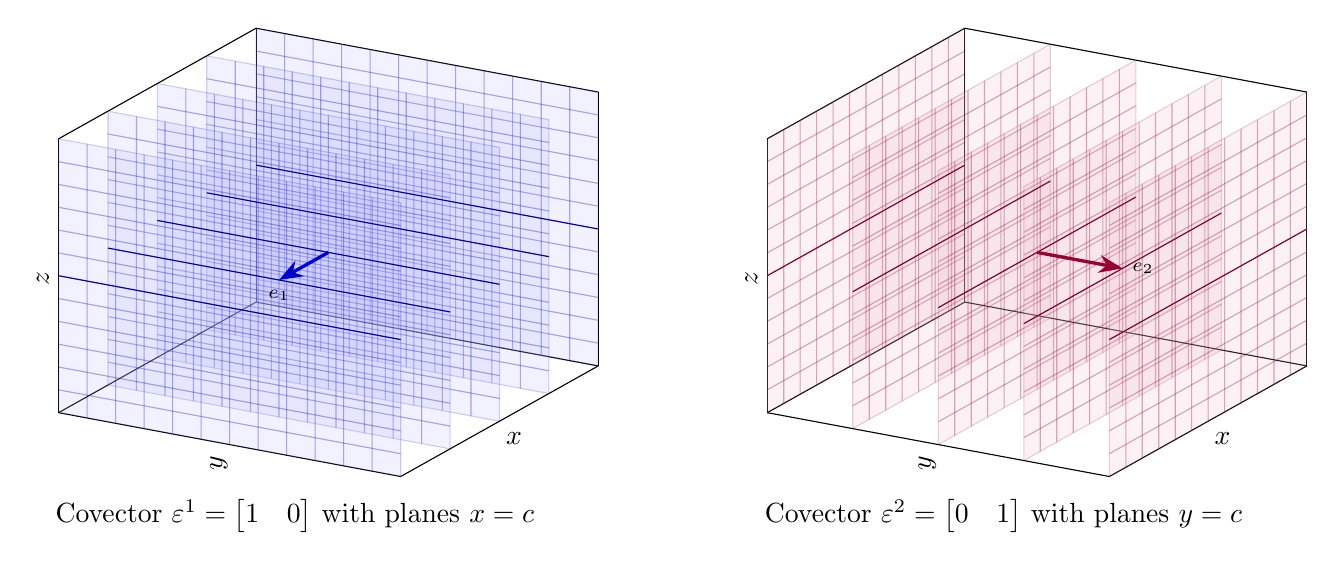
\begin{tikzpicture}	
\begin{axis}[
%	axis lines = middle,
	name=left,
	view={120}{25},
	axis lines=box, 
	ticks=none,
	xmin=-2, xmax=2, ymin=-2, ymax=2, zmin=-2, zmax=2,
	xlabel={$x$}, ylabel={$y$}, zlabel={$z$},
	]
	% A few planes x = c (literal constants)
	\addplot3[surf, opacity=0.18, draw=blue!70!black, fill=blue!30,
	shader=flat corner, domain=-2:2, y domain=-2:2, samples=13, samples y=13]
	({-2}, x, y);
	\addplot3[surf, opacity=0.18, draw=blue!70!black, fill=blue!30,
	shader=flat corner, domain=-2:2, y domain=-2:2, samples=13, samples y=13]
	({-1}, x, y);
	\addplot3[surf, opacity=0.18, draw=blue!70!black, fill=blue!30,
	shader=flat corner, domain=-2:2, y domain=-2:2, samples=13, samples y=13]
	({0},  x, y);
	\addplot3[surf, opacity=0.18, draw=blue!70!black, fill=blue!30,
	shader=flat corner, domain=-2:2, y domain=-2:2, samples=13, samples y=13]
	({1},  x, y);
	\addplot3[surf, opacity=0.18, draw=blue!70!black, fill=blue!30,
	shader=flat corner, domain=-2:2, y domain=-2:2, samples=13, samples y=13]
	({2},  x, y);
	\addplot3[blue!70!black] coordinates {(-2,-2,0) (-2,2,0)};
	\addplot3[blue!70!black] coordinates {(-1,-2,0) (-1,2,0)};
	\addplot3[blue!70!black] coordinates {( 0,-2,0) ( 0,2,0)};
	\addplot3[blue!70!black] coordinates {( 1,-2,0) ( 1,2,0)};
	\addplot3[blue!70!black] coordinates {( 2,-2,0) ( 2,2,0)};
	\addplot3[-{Stealth[length=3mm]}, very thick, blue!80!black]
	coordinates {(0,0,0) (1,0,0)};
	\node at (axis cs:1,0,0) [below, font=\scriptsize] {$e_1$};
\end{axis}
\node at (3,-.5) {Covector $\varepsilon^1=\begin{bmatrix}
		1 & 0
	\end{bmatrix}$ with planes $x=c$};
\begin{axis}[
	xshift=9cm,
	view={120}{25},
	axis lines=box, ticks=none,
	xmin=-2, xmax=2, ymin=-2, ymax=2, zmin=-2, zmax=2,
	xlabel={$x$}, ylabel={$y$}, zlabel={$z$},
	]
	% planes y = c (literal constants)
	\addplot3[surf, opacity=0.18, draw=purple!70!black, fill=purple!30,
	shader=flat corner, domain=-2:2, y domain=-2:2, samples=13, samples y=13]
	(x, {-2}, y);
	\addplot3[surf, opacity=0.18, draw=purple!70!black, fill=purple!30,
	shader=flat corner, domain=-2:2, y domain=-2:2, samples=13, samples y=13]
	(x, {-1}, y);
	\addplot3[surf, opacity=0.18, draw=purple!70!black, fill=purple!30,
	shader=flat corner, domain=-2:2, y domain=-2:2, samples=13, samples y=13]
	(x, {0},  y);
	\addplot3[surf, opacity=0.18, draw=purple!70!black, fill=purple!30,
	shader=flat corner, domain=-2:2, y domain=-2:2, samples=13, samples y=13]
	(x, {1},  y);
	\addplot3[surf, opacity=0.18, draw=purple!70!black, fill=purple!30,
	shader=flat corner, domain=-2:2, y domain=-2:2, samples=13, samples y=13]
	(x, {2},  y);
	\addplot3[purple!70!black] coordinates {(-2,-2,0) ( 2,-2,0)};
	\addplot3[purple!70!black] coordinates {(-2,-1,0) ( 2,-1,0)};
	\addplot3[purple!70!black] coordinates {(-2, 0,0) ( 2, 0,0)};
	\addplot3[purple!70!black] coordinates {(-2, 1,0) ( 2, 1,0)};
	\addplot3[purple!70!black] coordinates {(-2, 2,0) ( 2, 2,0)};
	\addplot3[-{Stealth[length=3mm]}, very thick, purple!80!black]
	coordinates {(0,0,0) (0,1,0)};
	\node at (axis cs:0,1,0) [right, font=\scriptsize] {$e_2$};
\end{axis}
\node at (12,-.5) {Covector $\varepsilon^2=\begin{bmatrix}
		0 & 1
	\end{bmatrix}$ with planes $y=c$};
\end{tikzpicture}
\end{center}

\newpage\noindent
Every vector \(\vec v\in V\) has a unique expansion \(\vec \vec{v}=\begin{bmatrix}
	v^1 \\ v^2
\end{bmatrix}=v^1 \vec{e}_1+v^2 \vec{e}_2\).
The dual basis \emph{reads off} these coordinates: \begin{align*}
	\varepsilon^1(\vec v)&=\varepsilon^1(v^1\vec{e}_1+v^2\vec{e}_2)=v^1\varepsilon^1(\vec{e}_1)+v^2\varepsilon^1(\vec{e}_2)=v_1, \\
	\varepsilon^2(\vec v)&=\varepsilon^2(v^1\vec{e}_1+v^2\vec{e}_2)=v^1\varepsilon^2(\vec{e}_1)+v^2\varepsilon^2(\vec{e}_2)=v_2.
\end{align*}
In matrix form, \[
\varepsilon^1(\vec{v})=\begin{bmatrix}1&0\end{bmatrix}\!\begin{bmatrix}v^1\\ v^2\end{bmatrix}=v^1,
\qquad
\varepsilon^2(\vec{v})=\begin{bmatrix}0&1\end{bmatrix}\!\begin{bmatrix}v^1\\ v^2\end{bmatrix}=v^2.
\]
For any \(\alpha\in V^*\) and \(\vec{v}=v^1 \vec{e}_1+v^2 \vec{e}_2\),
\[
\alpha(\vec v)
=\alpha(v^1 \vec{e}_1+v^2 \vec{e}_2)
= v^1\,\alpha(\vec{e}_1)+v^2\,\alpha(\vec{e}_2)
= \varepsilon^1(\vec v)\,\alpha(\vec{e}_1)+\varepsilon^2(\vec v)\,\alpha(\vec{e}_2).
\]
Set
\[
\alpha(\vec{e}_1)=\alpha_1\in\R,\qquad \alpha(\vec{e}_2)=\alpha_2\in\R.
\]
Then for every \(\vec v\in V\),
\[
\alpha(\vec v)=\alpha_1\,\varepsilon^1(\vec v)+\alpha_2\,\varepsilon^2(\vec v).
\]
Since this holds for all \(\vec v\), we identify \(\alpha\) as the linear combination
\[
\boxed{\ \alpha=\alpha_1\,\varepsilon^1+\alpha_2\,\varepsilon^2\ }\quad\in V^*.
\]
\begin{center}
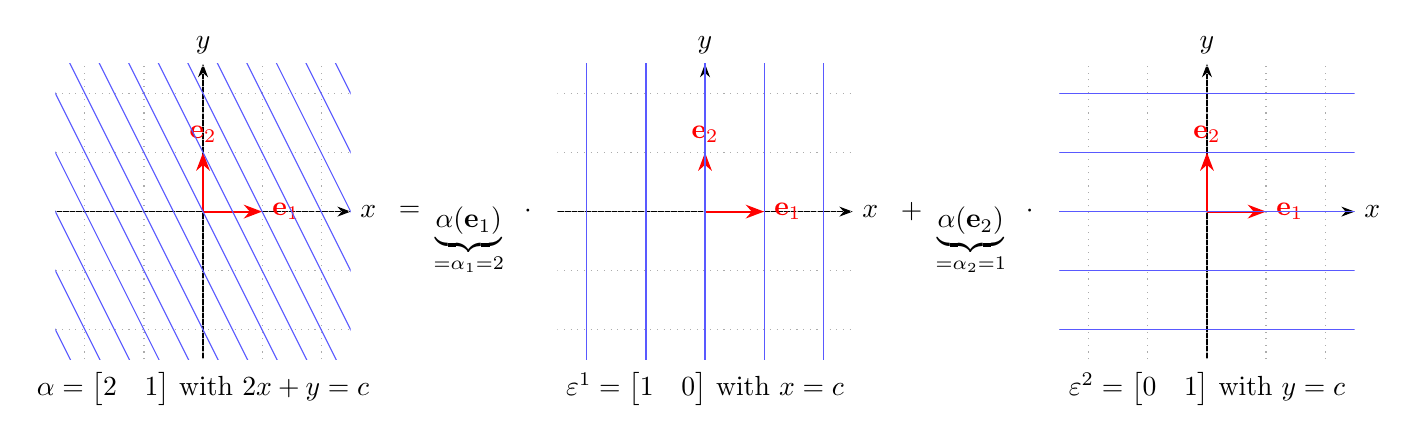
\begin{tikzpicture}[scale=.75, >=Stealth]
\draw[->] (-2.5,0) -- (2.5,0) node[right] {$x$};
\draw[->] (0,-2.5) -- (0,2.5) node[above] {$y$};
% Parallel level sets: 2x + y = c  (c from -3 to 3)
\begin{scope}
	\clip (-2.5,-2.5) rectangle (2.5,2.5); % (xmin,ymin) rectangle (xmax,ymax)
	\draw[dotted, gray!65] (-2.5,-2.5) grid (2.5,2.5);
	\draw[->, thick, red] (0,0) -- ++(1,0) node[right] {$\vec{e}_1$};
	\draw[->, thick, red] (0,0) -- ++(0,1) node[above] {$\vec{e}_2$};
	\foreach \c in {-14,-13,...,14}{
		\draw[blue!65] plot[domain=-10:10] (\x, {\c - 2*\x});
	}
\end{scope}
\node at (0,-3) {$\alpha=\begin{bmatrix} 2 & 1 \end{bmatrix}$ with $2x+y=c$};

\node at (3.5,0) {$=$};
\node at (4.5,-.5) {$\underbrace{\alpha(\vec{e}_1)}_{={\alpha_1}=2}$};
\node at (5.5,0) {$\cdot$};

\draw[->] (8.5+-2.5,0) -- (8.5+2.5,0) node[right] {$x$};
\draw[->] (8.5+0,-2.5) -- (8.5+0,2.5) node[above] {$y$};
\begin{scope}[xshift=8.5cm]
	\clip (-2.5,-2.5) rectangle (2.5,2.5); % (xmin,ymin) rectangle (xmax,ymax)
	\draw[dotted, gray!65] (-2.5,-2.5) grid (2.5,2.5);
	\draw[->, thick, red] (0,0) -- ++(1,0) node[right] {$\vec{e}_1$};
	\draw[->, thick, red] (0,0) -- ++(0,1) node[above] {$\vec{e}_2$};
	% Parallel level sets: 2x + y = c  (c from -3 to 3)
	\foreach \c in {-20,-19,...,20}{
		\draw[blue!65] plot[domain=-10:10] (\c, \x);
	}
\end{scope}
\node at (8.5,-3) {$\varepsilon^1=\begin{bmatrix} 1 & 0 \end{bmatrix}$ with $x=c$};

\node at (12,0) {$+$};
\node at (13,-.5) {$\underbrace{\alpha(\vec{e}_2)}_{={\alpha_2}=1}$};
\node at (14,0) {$\cdot$};

\draw[->] (17+-2.5,0) -- (17+2.5,0) node[right] {$x$};
\draw[->] (17+0,-2.5) -- (17+0,2.5) node[above] {$y$};
\begin{scope}[xshift=17cm]
	\clip (-2.5,-2.5) rectangle (2.5,2.5); % (xmin,ymin) rectangle (xmax,ymax)
	\draw[dotted, gray!65] (-2.5,-2.5) grid (2.5,2.5);
	\draw[->, thick, red] (0,0) -- ++(1,0) node[right] {$\vec{e}_1$};
	\draw[->, thick, red] (0,0) -- ++(0,1) node[above] {$\vec{e}_2$};
	% Parallel level sets: 2x + y = c  (c from -3 to 3)
	\foreach \c in {-14,-13,...,14}{
		\draw[blue!65] plot[domain=-10:10] (\x, \c);
	}
\end{scope}
\node at (17,-3) {$\varepsilon^2=\begin{bmatrix} 0 & 1 \end{bmatrix}$ with $y=c$};
\end{tikzpicture}
\end{center}

\newpage
\subsection{$\d x, \d y$ and $\d r, \d\theta$}

\begin{center}
\begin{tikzpicture}
\draw[-Stealth] (3,2) -- ++ (1,0) node[midway, above] {$\d$};
\draw[-Stealth] (12.2,2) -- ++ (1,0) node[midway, above] {$\d$};
\begin{groupplot}[
	group style={group size=4 by 1, horizontal sep=2.2cm},
	width=4.5cm, height=4cm,
	xmin=-2, xmax=2, ymin=-2, ymax=2,
	domain=-2:2, y domain=-2:2,
	colormap/cool,
	axis on top,
	]
	\nextgroupplot[
	title={Scalar field $x$},
	view={0}{90},
	axis equal image,
	xlabel={$x$}, ylabel={$y$},
	ticks=none,
	]
	\addplot3[
	surf, shader=interp,
	samples=45, samples y=45,
	] {x};
	
	\nextgroupplot[
	title={Covector field $\d x$},
	view={0}{90},
	axis equal image,
	xlabel={$x$}, ylabel={$y$},
	ticks=none,
	]		
	\addplot3[blue!70!black] coordinates {(0,-2,0) (0,2,0)};
	\addplot3[blue!70!black] coordinates {(1,-2,0) (1,2,0)};
	\addplot3[blue!70!black] coordinates {(-1,-2,0) (-1,2,0)};
	\addplot3[-Stealth, thick, blue] coordinates {(0,0,0) (0,1,0)} node[above] {$\partial_y$};
	\addplot3[-Stealth, thick, blue] coordinates {(0,0,0) (1,0,0)} node[right] {$\partial_x$};
	
	\nextgroupplot[
	title={Scalar field $y$},
	view={0}{90},
	axis equal image,
	xlabel={$x$}, ylabel={$y$},
	ticks=none,
	]
	\addplot3[
	surf, shader=interp,
	samples=45, samples y=45,
	] {y};
	
	\nextgroupplot[
	title={Covector field $\d y$},
	view={0}{90},
	axis equal image,
	xlabel={$x$}, ylabel={$y$},
	ticks=none,
	]		
	\addplot3[purple!70!black] coordinates {(-2,0,0) (2,0,0)};
	\addplot3[purple!70!black] coordinates {(-2,1,0) (2,1,0)};
	\addplot3[purple!70!black] coordinates {(-2,-1,0) (2,-1,0)};
	\addplot3[-Stealth, thick, purple] coordinates {(0,0,0) (0,1,0)} node[above] {$\partial_y$};
	\addplot3[-Stealth, thick, purple] coordinates {(0,0,0) (1,0,0)} node[right] {$\partial_x$};
\end{groupplot}
\end{tikzpicture}
\end{center}

\begin{center}
\begin{tikzpicture}
\draw[-Stealth] (3,2) -- ++ (1,0) node[midway, above] {$\d$};
\draw[-Stealth] (12.2,2) -- ++ (1,0) node[midway, above] {$\d$};
\begin{groupplot}[
	group style={group size=4 by 1, horizontal sep=2.2cm},
	width=4.5cm, height=4cm,
	xmin=-2, xmax=2, ymin=-2, ymax=2,
	domain=-2:2, y domain=-2:2,
	colormap/cool,
	axis on top,
	]
	\nextgroupplot[
		title={Scalar field $r$},
		view={0}{90},
		axis equal image,
		xlabel={$x$}, ylabel={$y$},
		ticks=none,
	] 		
	\addplot3[
		surf, shader=flat,           % flat = memory-friendly
		samples=45, samples y=45,    % keep modest; increase if you can
		domain=-2:2, y domain=-2:2,
	]{sqrt(x^2 + y^2)};
	
	\nextgroupplot[
		title={Covector field $\mathrm dr$},
		view={0}{90},
		axis equal image,
		xlabel={$x$}, ylabel={$y$},
		ticks=none,
	]
	\foreach \R in {1.0,2.0}{
		\addplot+[no marks, blue!70!black, domain=0:360, samples=121, variable=\t]
		({\R*cos(\t)},{\R*sin(\t)});
	}
%	\addplot[-stealth, thick, blue]
%	coordinates {(1,1) (1+0.55*0.83205, 1+0.55*0.55470)};
%	\addplot[-stealth, thick, teal!70!black]
%	coordinates {(1.2,0.8) (1.2-0.55*0.55470, 0.8+0.55*0.83205)};
	
	\nextgroupplot[
		title={Scalar field $\theta$},
		view={0}{90},
		axis equal image,
		xlabel={$x$}, ylabel={$y$},
		ticks=none,
	]
	\addplot3[
	surf, shader=flat,
	samples=45, samples y=45,
	domain=-2:2, y domain=-2:2,
	unbounded coords=discard         % skip undefined points near (0,0)
	] {atan2(y,x) * (pi/180)};
	% hide tiny undefined dot at origin
	\draw[fill=white, draw=none] (axis cs:0,0) circle[radius=0.04];
	
	\nextgroupplot[
	title={Covector field $\d\theta$},
	view={0}{90},
	axis equal image,
	xlabel={$x$}, ylabel={$y$},
	ticks=none,
	]
	\foreach \A in {0,20,...,340}{
		\addplot+[no marks, purple!70!black, domain=0:2, samples=2, variable=\r]
		({\r*cos(\A)},{\r*sin(\A)});
	}
	\addplot+[red!70, very thick] coordinates {(-2,0) (0,0)};
\end{groupplot}
\end{tikzpicture}
\end{center}

\begin{remark}[Parametrization for scalar field $\theta(x,y)$]
	Let \[
	x=r\cos t,\qquad y=r\sin t,\qquad r>0,\;t\in(-\pi,\pi].
	\] The scalar field $z=\theta(x,y)$ becomes the
	\emph{helicoid} parametrized by
	\[
	(r,t)\;\longmapsto\; (x,y,z=\theta(x,y))=\left(
		r\cos t,\;r\sin t,\;\theta(r\cos t,r\sin t)=\arctan\left(\frac{\sin t}{\cos t}\right)=\arctan(\tan(t))=t
	\right).
	\]
%	For fixed $t$ you get a \emph{generator} (straight line) on the surface; for fixed $r$
%	we get a \emph{helix} (wraps around as $t$ increases).
\end{remark}

%\begin{center}
%\begin{tikzpicture}[>=Stealth]
%
%% ===================== LEFT: y = tan x, y = x, y = arctan x =====================
%\begin{scope}[xshift=-4.8cm, scale=1.45]
%	\clip plot [] (-3.5,-2.4) rectangle (3.5, 2.4);
%	% Axes
%	\draw[->] (-1.9,0) -- (1.9,0) node[below right] {$x$};
%	\draw[->] (0,-3.5) -- (0,3.5) node[above left] {$y$};
%	
%	% Asymptotes for tan x at x = ± pi/2
%	\pgfmathsetmacro{\pih}{1.57079632679} % pi/2
%	\draw[gray!60,dashed] (\pih, -2.3) -- (\pih, 2.3);
%	\draw[gray!60,dashed] (-\pih, -2.3) -- (-\pih, 2.3);
%%	\draw[gray!60,dashed] (2*\pih, -2.3) -- (2*\pih, 2.3);
%%	\draw[gray!60,dashed] (-2*\pih, -2.3) -- (-2*\pih, 2.3);
%	\node[gray!70, font=\scriptsize] at (\pih, -2.2) {$x=\tfrac{\pi}{2}$};
%	\node[gray!70, font=\scriptsize] at (-\pih, -2.2) {$x=-\tfrac{\pi}{2}$};
%	
%	% y = tan x (principal branch), avoid endpoints
%	\draw[very thick, blue]
%	plot[samples=300, domain=-1.45:1.45] (\x, {tan(\x r)});
%	\node[blue, font=\scriptsize] at (1.2,2.1) {$y=\tan x$};
%	
%	% y = x
%	\draw[very thick, black!70]
%	plot[samples=2, domain=-1.8:1.8] (\x, {\x});
%	\node[black!70, font=\scriptsize] at (1.55,1.55) {$y=x$};
%	
%	% y = arctan x (atan returns degrees; convert to radians)
%	\draw[very thick, red!70!black]
%	plot[samples=300, domain=-1.8:1.8] (\x, {atan(\x)*(pi/180)});
%	\node[red!70!black, font=\scriptsize] at (1.5,0.6) {$y=\arctan x$};
%\end{scope}
%
%% ===================== RIGHT: plane picture for theta and dtheta =====================
%\begin{scope}[xshift=4.8cm, scale=1.45]
%	% Axes
%	\draw[->] (-2.4,0) -- (2.5,0) node[below right] {$x$};
%	\draw[->] (0,-2.4) -- (0,2.5) node[above left] {$y$};
%	% Rays (level sets of theta): theta = const
%	\foreach \ang in {0,20,40,60,80,100,120,140,160,180,200,220,240,260,280,300,320,340}{
%		\draw[gray!55] (0,0) -- ({2.2*cos(\ang)},{2.2*sin(\ang)});
%	}
%	% A sample point P and its triangle to axes
%	\coordinate (P) at (1.2,0.8); % x>0,y>0 so theta in (0,pi/2)
%	\fill (P) circle (1.1pt) node[above right] {$P=(x,y)$};
%	\draw[gray!70] (0,0) -- (P);
%	\draw[gray!70] (1.2,0) -- (P); % vertical leg
%	\draw[gray!70] (0,0) -- (1.2,0); % horizontal leg
%	% Right-angle marker
%	\draw[gray!70] (1.2,0) ++(-0.12,0) -- ++(0,0.12) -- ++(0.12,0);
%	
%	% Labels for legs (tan θ = y/x)
%	\node[font=\scriptsize] at (0.6,-0.18) {$x$};
%	\node[font=\scriptsize] at (1.35,0.42) {$y$};
%	
%	% Angle arc at origin for theta
%	\pgfmathsetmacro{\thetaDeg}{atan2(0.8,1.2)} % degrees
%	\draw[very thick, red!70!black] (0.45,0) arc (0:\thetaDeg:0.45);
%	\node[red!70!black, font=\scriptsize] at ({0.62*cos(\thetaDeg/2)},{0.62*sin(\thetaDeg/2)}) {$\theta$};
%	
%	% dtheta visualization: small arc arrow at radius r0 shows infinitesimal change
%	\pgfmathsetmacro{\rzero}{1.6}
%	\draw[very thick, orange!80!black, -{Stealth[length=2mm]}]
%	({\rzero*cos(\thetaDeg)},{\rzero*sin(\thetaDeg)})
%	arc (\thetaDeg:{\thetaDeg+14}:{\rzero});
%	\node[font=\scriptsize, orange!80!black, fill=white, inner sep=1pt]
%	at ({\rzero*cos(\thetaDeg+7)},{\rzero*sin(\thetaDeg+7)}) {$d\theta$};
%	
%	% Show that dθ kills radial motion and measures angular motion:
%	% radial arrow (dr != 0, dθ = 0)
%	\draw[very thick, blue!70, -{Stealth[length=2mm]}]
%	({1.4*cos(\thetaDeg)},{1.4*sin(\thetaDeg)})
%	-- ++({0.5*cos(\thetaDeg)},{0.5*sin(\thetaDeg)});
%	\node[font=\scriptsize, blue!70] at ({1.65*cos(\thetaDeg)},{1.65*sin(\thetaDeg)-0.15})
%	{$dr\neq 0,\ d\theta=0$};
%	
%	% angular arrow (dr = 0, dθ != 0) tangent to the circle
%	\draw[very thick, teal!70!black, -{Stealth[length=2mm]}]
%	({1.4*cos(\thetaDeg)},{1.4*sin(\thetaDeg)})
%	-- ++({-0.5*sin(\thetaDeg)},{0.5*cos(\thetaDeg)});
%	\node[font=\scriptsize, teal!70!black] at ({1.4*cos(\thetaDeg)-0.35*sin(\thetaDeg)},{1.4*sin(\thetaDeg)+0.35*cos(\thetaDeg)+0.15})
%	{$dr=0,\ d\theta\neq 0$};
%\end{scope}
%\end{tikzpicture}
%\end{center}
%
%\begin{tikzpicture}
%	\begin{axis}[
%		title={Scalar field $\theta(x,y)=\arctan(y/x)$},
%		view={0}{90}, axis equal image,
%		xmin=-2, xmax=2, ymin=-2, ymax=2,
%		xlabel={$x$}, ylabel={$y$},
%		ticks=none,
%		point meta=z,
%		colormap/cool,
%		colorbar,
%		colorbar style={
%%			ylabel={$\theta$ (rad)},
%			ytick={-3.1416,-1.5708,0,1.5708,3.1416},
%			yticklabels={$-\pi$,$-\frac{\pi}{2}$,$0$,$\frac{\pi}{2}$,$\pi$},
%		},
%		]
%		% Lighter mesh + flat shader = much lower memory
%		\addplot3[
%		surf, shader=flat,      % flat shading is light on memory
%		samples=41, samples y=41, % keep this modest (41–61)
%		domain=-2:2, y domain=-2:2,
%		unbounded coords=discard % avoid NaNs near (0,0)
%		] {atan2(y,x)*(pi/180)};   % atan2 returns degrees → convert to radians
%		% Hide a tiny disk at the undefined origin
%		\draw[fill=white, draw=none] (axis cs:0,0) circle[radius=0.04];		
%		% (Optional) faint rays to suggest level sets of theta
%%		\foreach \A in {0,30,...,330}{
%%			\addplot3[gray!55, thin] coordinates {(0,0,0) ({2*cos(\A)},{2*sin(\A)},0)};
%%		}
%	\end{axis}
%\end{tikzpicture}

\newpage
%\subsection{The Surface $z=\theta(x,y)$ with $\theta=\operatorname{atan2}(y/x)$}
\subsection{The surface $z=\theta(x,y)$}
We visualize the scalar field $z \;=\; \theta(x,y)$ as a surface:
\begin{center}
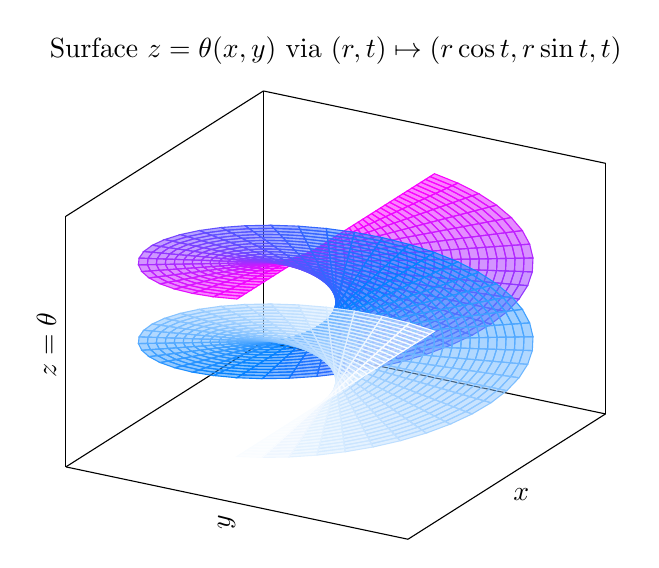
\begin{tikzpicture}[scale=1]
	\begin{axis}[
%		title={Surface $z=\theta(x,y)$ with $(x,y)=(r\cos t,r\sin t)$ and $z=t$},
		title={Surface $z=\theta(x,y)$ via $(r,t)\mapsto(r\cos t,r\sin t,t)$},
		view={120}{30},
		xlabel={$x$}, ylabel={$y$}, zlabel={$z=\theta$},
		axis lines=box, 
		ticks=none,
		xmin=-2.5, xmax=2.5, ymin=-2.5, ymax=2.5, zmin=-5, zmax=5,
		colormap/cool
		]
		% Parametric surface: (X,Y,Z) = (r cos t, r sin t, t)
		% Use degrees for trig to avoid deg<->rad conversions in every sample:
		% y parameter = t_deg ∈ [-180,180], so z = t = t_deg * pi/180.
		\addplot3[
		surf,
%		draw=white, 
		fill opacity=.5,     % wireframe only (no fill)
		shader=flat,                       % cheap
		samples=45, samples y=45,          % modest grid; raise slightly if desired
		domain=-2.5:2.5,                   % skip tiny disk around the singularity
		y domain=-180:180
		] ({x*cos(y)}, {x*sin(y)}, {y*pi/180});
	\end{axis}
\end{tikzpicture}
\end{center}
%On $\mathbb{R}^2\setminus\{0\}$,
%\[
%\d\theta \;=\; \frac{-y\,\d x + x\,\d y}{x^2+y^2},\qquad
%\nabla \theta \;=\; \left(-\frac{y}{x^2+y^2},\;\frac{x}{x^2+y^2}\right).
%\]
%The gradient $\nabla\theta$ is \emph{perpendicular to the radial direction} $(x,y)$ and tangent to circles around the origin, with magnitude $\|\nabla\theta\|=1/\sqrt{x^2+y^2}$.
We identify the plane $\mathbb{R}^2$ with the complex line $\mathbb{C}$ via
\[
(x,y)\ \longleftrightarrow\ z:=x+iy.
\]
%For $z\neq 0$ let $r=|z|=\sqrt{x^2+y^2}$. The \emph{geometric angle}
%$\theta(x,y)$ of $(x,y)$ is the signed angle from the positive $x$-axis to the
%vector $(x,y)$.
\begin{center}
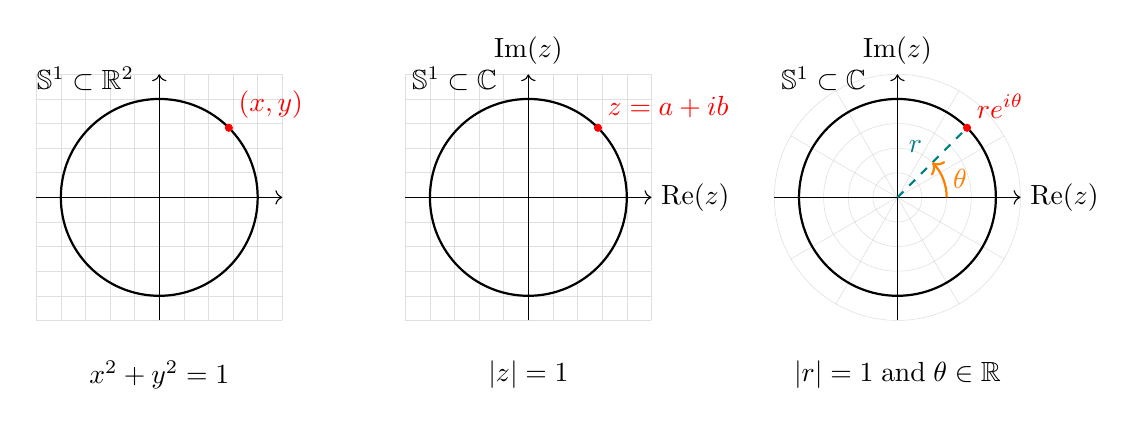
\begin{tikzpicture}[scale=1.25]
% Left illustration: R^2 representation of the unit circle
\begin{scope}[xshift=0cm]
	\draw[step=.25cm,gray!50,very thin,opacity=.5] (-1.25,-1.25) grid (1.25,1.25);
	% Axes for R^2
	\draw[->] (-1.25,0) -- (1.25,0) node[right] {$\R$};
	\draw[->] (0,-1.25) -- (0,1.25) node[above] {$\R$};
	% The unit circle in R^2
	\draw[thick] (0,0) circle (1cm);
	% Label the circle with its equation
	\node at (0,-1.8) {\(x^2 + y^2 = 1\)};
	\node at (-.75,1.2) {\(\mathbb{S}^1 \subset \mathbb{R}^2\)};
	\filldraw[red] (45:1cm) circle (1pt) node[above right] {\((x,y)\)};
\end{scope}
% Right illustration: Complex plane representation of the unit circle
\begin{scope}[xshift=3.75cm]
	\draw[step=.25cm,gray!50,very thin,opacity=.5] (-1.25,-1.25) grid (1.25,1.25);
	% Axes for the complex plane
	\draw[->] (-1.25,0) -- (1.25,0) node[right] {\(\Re(z)\)};
	\draw[->] (0,-1.25) -- (0,1.25) node[above] {\(\Im(z)\)};
	% The unit circle in the complex plane
	\draw[thick] (0,0) circle (1cm);
	% Draw an arc to indicate the angle theta
	%		\draw[->, red] (0.5,0) arc (0:45:0.5);
	%		\node at (0.7,0.2) {\(\theta\)};
	% Mark and label a point on the circle corresponding to e^(i theta)
	\filldraw[red] (45:1cm) circle (1pt) node[above right] {\(z = a + ib\)};
	% Label the circle with its modulus condition
	\node at (0,-1.8) {\(|z| = 1\)};
	\node at (-.75,1.2) {\(\mathbb{S}^1 \subset \mathbb{C}\)};
	
	%		\filldraw[red] (1,1) circle (1.5pt) node[anchor=south west, black] {$$};
\end{scope}
\begin{scope}[xshift=7.5cm]
	% Draw concentric circles for radii 1 to 5
	\foreach \r in {.25,.5,...,1.25} {
		\draw[very thin, gray!50, opacity=.5] (0,0) circle (\r);
	}
	% Draw radial lines at every 30 degrees
	\foreach \angle in {0,30,...,360} {
		\draw[very thin, gray!50, opacity=.5] (0,0) -- (\angle:1.25);
	}
	
	% Axes for the complex plane
	\draw[->] (-1.25,0) -- (1.25,0) node[right] {\(\Re(z)\)};
	\draw[->] (0,-1.25) -- (0,1.25) node[above] {\(\Im(z)\)};
	% The unit circle in the complex plane
	\draw[thick] (0,0) circle (1cm);
	% Draw an arc to indicate the angle theta
	%		\draw[->, red] (0.5,0) arc (0:45:0.5);
	%		\node at (0.7,0.2) {\(\theta\)};
	% Mark and label a point on the circle corresponding to e^(i theta)
	\filldraw[red] (45:1cm) circle (1pt) node[above right] {\(re^{i\theta}\)};
	% Label the circle with its modulus condition
	\node at (0,-1.8) {\(\abs{r}=1\;\text{and}\;\theta \in \mathbb{R}\)};
	\node at (-.75,1.2) {\(\mathbb{S}^1 \subset \mathbb{C}\)};
	% draw radius
	\draw[dashed, thick, teal] (0,0) -- (.71,0.71) node[midway, above left] {$r$};
	% draw angle
	\draw[->, thick, orange] (0.5,0) arc (0:45:0.5) node[midway, right] {$\theta$};
\end{scope}
\end{tikzpicture}
\end{center}

\newpage
The one-argument arctangent \[
\arctan:\mathbb{R}\to(-\frac{\pi}{2},\frac{\pi}{2})
\] is single-valued but \emph{cannot} return angles outside that range. The correct globally defined angle (mod $2\pi$), with a chosen principal branch, is given by the two-argument arctangent:
\[
\theta=\operatorname{atan2}(y,x)\in(-\pi,\pi],
\]
which is defined piecewise by
\[
\theta=
\begin{cases}
	\arctan\!\big(\tfrac{y}{x}\big), & x>0,\\[4pt]
	\arctan\!\big(\tfrac{y}{x}\big)+\pi, & x<0,\ y\ge 0,\\[4pt]
	\arctan\!\big(\tfrac{y}{x}\big)-\pi, & x<0,\ y<0,\\[4pt]
	\ \ \frac{\pi}{2}, & x=0,\ y>0,\\[4pt]
	-\frac{\pi}{2}, & x=0,\ y<0,
\end{cases}
\quad\text{(undefined at $x=y=0$).}
\]


Hence:
\[
\boxed{\ \text{Global angle (principal): }\ \theta(x,y)=\operatorname{atan2}(y,x). \ }
\]
On the right half-plane $x>0$ this reduces to the simple formula $\arctan(y/x)$.

\section*{3. Complex viewpoint: \texorpdfstring{$\Arg$}{Arg} of a complex number}
Write $z=x+iy\in\mathbb{C}^\times$. The (principal) argument $\Arg z\in(-\pi,\pi]$ is defined by the \emph{polar form}
\[
z=|z|\,e^{i\,\Arg z}.
\]
Equivalently,
\[
\frac{z}{|z|}=\cos(\Arg z)+i\sin(\Arg z).
\]
Thus the geometric angle $\theta(x,y)$ is the principal argument:
\[
\boxed{\ \theta(x,y)=\Arg(x+iy)=\operatorname{atan2}(y,x). \ }
\]
This is the cleanest global statement; it automatically handles all quadrants
and the axes (except the origin).

\section*{4. When does \texorpdfstring{$\arctan(y/x)$}{arctan(y/x)} equal the true angle?}
Let $\theta=\Arg(x+iy)\in(-\pi,\pi]$. Then:
\[
\arctan\!\Big(\frac{y}{x}\Big)=\theta
\quad\Longleftrightarrow\quad
\theta\in\Big(-\frac{\pi}{2},\frac{\pi}{2}\Big)\ \text{(i.e.\ $x>0$)}.
\]
In general,
\[
\arctan\!\Big(\frac{y}{x}\Big)=\theta - \pi\,N,\qquad
N=\left\lfloor \frac{\theta}{\pi}+\frac12\right\rfloor\in\{-1,0,1\}.
\]
The subtracted multiple of $\pi$ compensates for the quadrant.

\section*{5. Analytic formula via the complex logarithm}
For a \emph{complex} variable $w$, the complex arctangent is defined (on a
log-branch domain) by
\[
\arctan w \;=\; \frac{1}{2i}\,\Big(\log(1+i w)-\log(1-i w)\Big),
\]
where $\log$ is a chosen branch of the complex logarithm. This identity is
obtained by differentiating both sides and matching values at $w=0$. Its branch
cuts are typically placed so that $1\pm i w$ avoid the logarithm’s cut.

\paragraph{Specialization to $w=\dfrac{y}{x}$ (real ratio).}
When $x\neq 0$ and $w=y/x\in\mathbb{R}$, the above produces the real
$\arctan(w)\in(-\tfrac{\pi}{2},\tfrac{\pi}{2})$. But to recover the \emph{global}
geometric angle you must still correct by $\pm \pi$ according to the sign of $x$
(i.e.\ use $\operatorname{atan2}$), or, equivalently, use $\Arg(x+iy)$ directly.

\section*{6. Branch cuts and continuity of the angle}
Any single-valued selection of the angle on $\mathbb{R}^2\setminus\{0\}$ must jump by $2\pi$ somewhere (a \emph{branch cut}). The standard choice (principal branch) places the cut along the negative real axis:
\[
\Arg:\ \mathbb{C}\setminus(-\infty,0]\ \longrightarrow\ (-\pi,\pi].
\]
Crossing the cut increases/decreases the angle by $2\pi$. This is why a color
plot of $\theta(x,y)$ shows a “seam” along $x<0,y=0$.

\section*{7. Differential of the angle and the 1-form \texorpdfstring{$d\theta$}{dθ}}
From
\[
z=|z|e^{i\theta}\quad\Longrightarrow\quad d(\log z)=\frac{dz}{z}
=d(\ln|z|)+i\,d\theta,
\]
and writing $z=x+iy$, $dz=dx+i\,dy$, we get
\[
\frac{dz}{z}
=\frac{dx+i\,dy}{x+iy}
=\frac{(x\,dx+y\,dy)+i(x\,dy-y\,dx)}{x^2+y^2}.
\]
Taking imaginary parts:
\[
\boxed{\ d\theta=\frac{x\,dy-y\,dx}{x^2+y^2}\qquad (x,y)\neq(0,0).\ }
\]
Geometrically:
\begin{itemize}
	\item $d\theta$ vanishes on \emph{radial} motion (along rays $\theta=\text{const}$).
	\item $d\theta$ measures \emph{angular} motion (tangent to circles).
\end{itemize}
For a closed loop $\gamma$ avoiding $0$,
\[
\int_\gamma d\theta = 2\pi\,\mathrm{Ind}(\gamma,0),
\]
the net number of turns around the origin (winding number).

\section*{8. Examples and edge cases}
\begin{itemize}
	\item $(x,y)=(1,1)$: $\arctan(y/x)=\arctan(1)=\pi/4$; $\Arg(1+i)=\pi/4$ (agree).
	\item $(x,y)=(-1,1)$: $\arctan(y/x)=\arctan(-1)=-\pi/4$ but the true angle is
	$3\pi/4$. Here $\operatorname{atan2}(1,-1)=3\pi/4=\arctan(-1)+\pi$.
	\item $(x,y)=(0,-2)$: $\arctan(y/x)$ undefined; $\operatorname{atan2}(-2,0)=-\pi/2$;
	$\Arg(-2i)=-\pi/2$.
	\item $(x,y)=(-3,0)$: slope $0$ so $\arctan(0)=0$ (misleading);
	$\operatorname{atan2}(0,-3)=\pi$; $\Arg(-3)=\pi$ (principal).
\end{itemize}

\section*{9. A precise dictionary}
\begin{itemize}
	\item \textbf{Local/right half-plane formula:}
	\[
	\theta=\arctan(y/x)\quad\text{(valid for $x>0$).}
	\]
	\item \textbf{Global/principal angle:}
	\[
	\theta=\operatorname{atan2}(y,x)=\Arg(x+iy)\in(-\pi,\pi].
	\]
	\item \textbf{Complex-analytic identity:} for $w\in\mathbb{C}$,
	\[
	\arctan w=\frac{1}{2i}\Big(\log(1+iw)-\log(1-iw)\Big)
	\]
	(on a suitable log-branch domain).
	\item \textbf{Differential:}
	\[
	d\theta=\dfrac{x\,dy-y\,dx}{x^2+y^2}=\Im\!\left(\dfrac{dz}{z}\right).
	\]
\end{itemize}

\section*{10. Common pitfalls (and remedies)}
\begin{itemize}
	\item Using $\arctan(y/x)$ globally \emph{without} correcting the quadrant.
	Remedy: use $\operatorname{atan2}(y,x)$ or $\Arg(x+iy)$.
	\item Forgetting the point $(0,0)$ is excluded; $\theta$ and $d\theta$ are not defined there.
	\item Expecting a continuous single-valued $\theta$ on the punctured plane
	\emph{without} a branch cut. Any single-valued angle has a jump by $2\pi$
	along some cut.
	\item Confusing degrees and radians: in plotting packages $\operatorname{atan2}$
	often returns \emph{degrees}; multiply by $\pi/180$ to get radians.
\end{itemize}

\newpage
\section*{1. Argument as a scalar field on $\C^\times$}
For $z=x+iy\in\C^\times=\C\setminus\{0\}$, write $z=re^{i\theta}$ with
\[
r=|z|=\sqrt{x^2+y^2},\qquad \theta=\arg z \in \R/2\pi\mathbb{Z}.
\]
Any \emph{single-valued} choice of $\theta$ requires a \emph{branch cut}. The
\emph{principal argument} is
\[
\Arg z \in (-\pi,\pi],\qquad \text{cut usually along } (-\infty,0)\subset\R.
\]
In coordinates, $\Arg(x+iy)$ coincides with the quadrant-aware angle $\operatorname{atan2}(y,x)$.
(Using $\arctan(y/x)$ \emph{without} quadrant care is ambiguous on $x<0$.)

\paragraph{Level sets.} For fixed $\theta_0$, the set $\{z\neq0:\arg z=\theta_0\}$ is the \emph{ray}
$\{re^{i\theta_0}: r>0\}$.

\section*{2. Relation to the complex logarithm}
On a simply connected domain avoiding $0$ and the cut, define a holomorphic branch of the log:
\[
\Log z = \ln|z| + i\,\Arg z = u + iv, \qquad u=\ln r,\ v=\Arg z.
\]
Then $\theta=\Arg z=\Im(\Log z)$ and
\[
d(\Log z)=\frac{dz}{z},\qquad \Im\!\big(d(\Log z)\big)=d\theta.
\]

\section*{3. Differential and gradient}
With $z=x+iy$ and $dz=dx+i\,dy$,
\[
\frac{dz}{z} = \frac{dx+i\,dy}{x+iy}
= \frac{(x\,dx+y\,dy)+i(x\,dy-y\,dx)}{x^2+y^2}.
\]
Hence
\[
\boxed{\,d\theta = \Im\!\left(\frac{dz}{z}\right) = \frac{x\,dy-y\,dx}{x^2+y^2}\,}
\quad\text{on }\C^\times.
\]
In the Euclidean metric, the gradient of $\theta$ is
\[
\boxed{\,\nabla\theta(x,y) = \left(\!-\,\frac{y}{x^2+y^2},\ \frac{x}{x^2+y^2}\right),\qquad
	\|\nabla\theta\| = \frac{1}{\sqrt{x^2+y^2}}=\frac{1}{r}\, .}
\]
Thus $\nabla\theta$ is \emph{tangent to circles} and \emph{orthogonal to the radius}.

\section*{4. Winding number via a line integral}
For a closed $C^1$ curve $\gamma$ avoiding $0$,
\[
\int_\gamma d\theta
= \Im\!\int_\gamma \frac{dz}{z}
= 2\pi\,\mathrm{Ind}(\gamma,0),
\]
the net angle (in radians) swept by the radius vector as you traverse $\gamma$.
Equivalently, $\displaystyle\int_\gamma \frac{dz}{z}=2\pi i\,\mathrm{Ind}(\gamma,0)$.

\paragraph{Example (unit circle).}
Let $\gamma(t)=e^{it}$, $t\in[0,2\pi]$. Then $dz/z = i\,dt$, so
\[
\int_\gamma d\theta
= \Im\!\int_0^{2\pi} i\,dt
= \Im\,[2\pi i]
= 2\pi,
\]
which is the expected one full turn around the origin.

\section*{5. Harmonic conjugates and Cauchy--Riemann}
On a branch domain, $u=\ln r$ and $v=\theta$ satisfy Cauchy--Riemann and are harmonic:
\[
\Delta u=0,\qquad \Delta v=0\quad\text{on }\C^\times,\qquad
\nabla v = J\,\nabla u,\ \ J=\begin{bmatrix}0&-1\\ 1&0\end{bmatrix}.
\]
So $\nabla(\ln r)=\dfrac{1}{r^2}(x,y)$ is radial, while $\nabla\theta=\dfrac{1}{r^2}(-y,x)$ is the $+\pi/2$ rotation of it.

\bigskip\hrule\bigskip

\section*{6. Two compact TikZ visuals}

\subsection*{(A) Branch cut and level sets of $\theta$ (rays)}
\begin{center}
	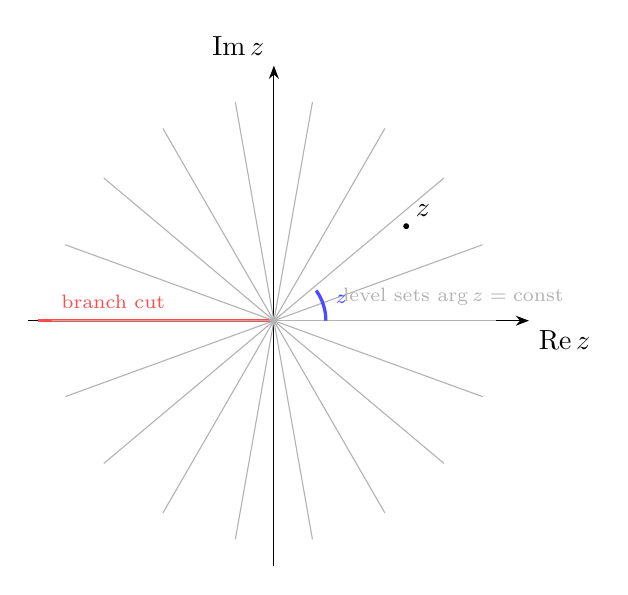
\begin{tikzpicture}[scale=1.2,>=Stealth]
		% Axes
		\draw[->] (-2.6,0) -- (2.7,0) node[below right] {$\Re z$};
		\draw[->] (0,-2.6) -- (0,2.7) node[above left] {$\Im z$};
		
		% Branch cut on negative real axis
		\draw[very thick, red!70] (-2.5,0) -- (0,0);
		\node[red!70, font=\scriptsize] at (-1.7,0.2) {branch cut};
		
		% Rays (level sets of theta)
		\foreach \ang in {0,20,40,60,80,100,120,140,160,180,200,220,240,260,280,300,320,340}{
			\draw[gray!60] (0,0) -- ({2.35*cos(\ang)},{2.35*sin(\ang)});
		}
		\node[font=\scriptsize,gray!60] at (1.9,0.25) {level sets $\arg z=\text{const}$};
		
		% Sample point and its angle
		\coordinate (P) at (1.4,1.0);
		\fill (P) circle (0.9pt) node[above right] {$z$};
		\pgfmathsetmacro{\th}{atan2(1.0,1.4)}
		\draw[very thick, blue!70] (0.55,0) arc (0:\th:0.55);
		\node[blue!70, font=\scriptsize] at ({0.75*cos(\th/2)},{0.75*sin(\th/2)}) {$\Arg z$};
	\end{tikzpicture}
\end{center}

\subsection*{(B) Gradient field $\nabla\theta$ (tangent to circles)}
\begin{center}
	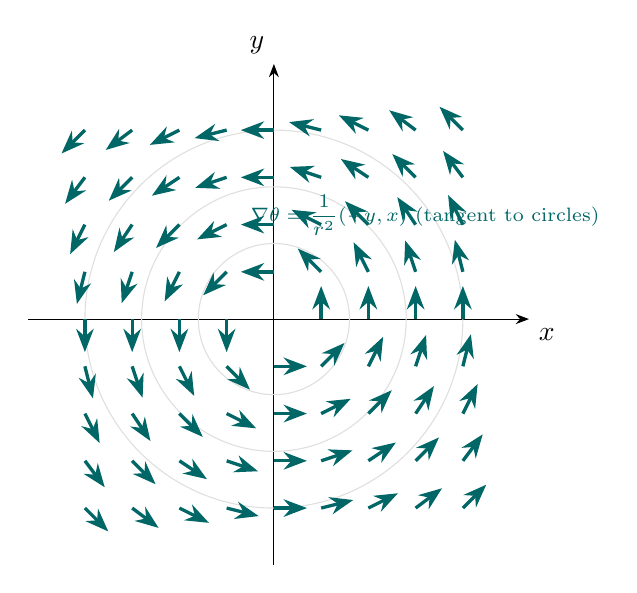
\begin{tikzpicture}[scale=1.2,>=Stealth]
		% Axes
		\draw[->] (-2.6,0) -- (2.7,0) node[below right] {$x$};
		\draw[->] (0,-2.6) -- (0,2.7) node[above left] {$y$};
		
		% Light circles (context)
		\foreach \R in {0.8,1.4,2.0}{
			\draw[gray!25] (0,0) circle (\R);
		}
		
		% Gradient vectors (normalized to constant display length)
		\foreach \xx in {-2.0,-1.5,-1.0,-0.5,0,0.5,1.0,1.5,2.0}{
			\foreach \yy in {-2.0,-1.5,-1.0,-0.5,0,0.5,1.0,1.5,2.0}{
				\pgfmathsetmacro{\r}{sqrt(\xx*\xx+\yy*\yy)}
				\ifdim \r pt > 0.25pt
				\pgfmathsetmacro{\ux}{-\yy/\r}
				\pgfmathsetmacro{\uy}{ \xx/\r}
				\draw[->, very thick, teal!80!black] (\xx,\yy) -- ++({0.35*\ux},{0.35*\uy});
				\fi
			}
		}
		
		\node[font=\scriptsize,teal!80!black] at (1.6,1.1)
		{$\nabla\theta=\dfrac{1}{r^2}(-y,x)$ (tangent to circles)};
	\end{tikzpicture}
\end{center}

\bigskip\hrule\bigskip

\section*{7. Quick dictionary}
\begin{itemize}
	\item \(\arg z\): multi-valued angle; \(\mathrm{Arg}\,z\) is a single-valued branch (needs a cut).
	\item \(\Log z=\ln|z|+i\,\Arg z\) (holomorphic on a branch domain), \(d\Log z=\dfrac{dz}{z}\).
	\item \(d\theta=\Im\!\left(\dfrac{dz}{z}\right)=\dfrac{x\,dy-y\,dx}{x^2+y^2}\).
	\item \(\displaystyle \int_\gamma d\theta = 2\pi\,\mathrm{Ind}(\gamma,0)\) (net turning / winding number).
	\item \(u=\ln r\) and \(v=\theta\) are harmonic conjugates: \(u+iv=\Log z\).
\end{itemize}


%\begin{tikzpicture}
%	\begin{axis}[
%		title={Gradient field of $\theta(x,y)=\operatorname{atan2}(y,x)$},
%		axis equal image,
%		view={0}{90},              % top-down
%		xmin=-2, xmax=2, ymin=-2, ymax=2,
%		xlabel={$x$}, ylabel={$y$},
%		ticks=none
%		]
%		
%%		% (Optional) very light scalar-field heatmap for context (flat shader, modest samples)
%%		\addplot3[
%%		surf, shader=flat,
%%		samples=41, samples y=41,
%%		domain=-2:2, y domain=-2:2,
%%		colormap/viridis, point meta=z, forget plot
%%		] {atan2(y,x)*(pi/180)};
%%		% Hide tiny disk at the undefined origin
%%		\draw[fill=white, draw=none] (axis cs:0,0) circle[radius=0.04];
%%		
%%		% (Optional) faint rays showing level sets theta = const
%%		\foreach \A in {0,30,...,330}{
%%			\addplot3[gray!55, thin, forget plot]
%%			coordinates {(0,0,0) ({2*cos(\A)},{2*sin(\A)},0)};
%%		}
%		
%		% ===== Gradient vector field: ∇θ = (-y/(x^2+y^2), x/(x^2+y^2)) =====
%		% Use quiver with expressions in x,y. To avoid the (0,0) singularity,
%		% normalize with r = sqrt(x^2+y^2 + eps) so arrows have ~constant length.
%%		\addplot[
%%		quiver={
%%			u={-y/sqrt(x^2+y^2 + 1e-6)},   % direction tangent to circle
%%			v={ x/sqrt(x^2+y^2 + 1e-6)},   % (≈ normalized ∇θ)
%%			scale arrows=0.28
%%		},
%%		-stealth, very thick, blue!70!black,
%%		samples=15, samples y=15,
%%		domain=-2:2, y domain=-2:2
%%		] (x,y);
%
%		\addplot[		
%		title={Gradient field $\nabla f=\langle 2,1\rangle$},
%		view={0}{90},
%		axis equal image,
%		xlabel={$x$}, ylabel={$y$},
%		ticks=none,
%		]		
%		% Gradient field arrows: (2x, 2y)
%		\addplot3[
%		-stealth,
%		quiver={
%			u={-y/sqrt(x^2+y^2 + 1e-6)}, v={ x/sqrt(x^2+y^2 + 1e-6)}, w=0,
%			scale arrows=0.12
%		},
%		samples=16,
%		samples y=16,
%		domain=-2:1.8, y domain=-2:1.8,
%		] ({x},{y},{0});
%		
%	\end{axis}
%\end{tikzpicture}


\begin{tikzpicture}[>=Stealth, scale=1.35]
	
	% Axes
	\draw[->] (-2.6,0) -- (2.7,0) node[below right] {$x$};
	\draw[->] (0,-2.6) -- (0,2.7) node[above left] {$y$};
	
	% Title / formulas
	\node[anchor=south west, font=\small] at (-2.55,2.55)
	{$\displaystyle \theta(x,y)=\arctan\!\Big(\frac{y}{x}\Big),\quad
		\nabla\theta=\Big(\frac{-y}{x^2+y^2},\,\frac{x}{x^2+y^2}\Big),\quad
		d\theta=\frac{-y\,dx+x\,dy}{x^2+y^2}$};
	
	% Rays = level sets theta = const
	\foreach \ang in {0,15,...,345}{
		\draw[gray!60] (0,0) -- ({2.4*cos(\ang)},{2.4*sin(\ang)});
	}
	\node[gray!60, font=\scriptsize] at (2.1,0.25) {level sets $\theta=\text{const}$ (rays)};
	
	% A few circles to suggest polar grid (not level sets of theta, just context)
	\foreach \R in {0.8,1.4,2.0}{
		\draw[gray!25] (0,0) circle (\R);
	}
	
	% Choose a sample point P (x>0,y>0 so theta in (0,pi/2))
	\coordinate (P) at (1.5,0.9);
	\fill (P) circle (1.0pt) node[above right] {$P=(x,y)$};
	
	% Angle arc at origin showing theta
	\pgfmathsetmacro{\thetaDeg}{atan2(0.9,1.5)} % degrees
	\draw[very thick, red!70!black] (0.55,0) arc (0:\thetaDeg:0.55);
	\node[red!70!black, font=\scriptsize]
	at ({0.75*cos(\thetaDeg/2)},{0.75*sin(\thetaDeg/2)}) {$\theta$};
	
	% Radial vector at P (points from origin to P)
	\draw[very thick, blue!70, -{Stealth[length=2.2mm]}] (0,0) -- (P)
	node[midway, below right, font=\scriptsize] {radial};
	
	% Gradient vector at P: proportional to (-y, x) / r^2 (draw a scaled version for clarity)
	% Compute a small multiple of (-y, x) for a neat arrow length:
	\pgfmathsetmacro{\gx}{-0.8*0.9}  % -k*y
	\pgfmathsetmacro{\gy}{ 0.8*1.5}  %  k*x
	\draw[very thick, orange!85!black, -{Stealth[length=2.2mm]}] (P) -- ++(\gx,\gy)
	node[above right, xshift=2pt, font=\scriptsize] {$\nabla\theta\ \perp\ (x,y)$};
	
	% Tangent direction label (showing perpendicularity)
	\draw[densely dashed, orange!70]
	($(P)+(\gx*0.65,\gy*0.65)$) -- ($(P)-(\gx*0.25,\gy*0.25)$);
	\node[font=\scriptsize, fill=white, inner sep=1pt]
	at ($(P)+(\gx*0.4,\gy*0.4)+(0.0,0.15)$) {tangent to circle};
	
	% dθ glyphs: short segments aligned with the rays (the directions dθ "kills")
	\foreach \ang in {10,40,70,100,130,160,190,220,250,280,310,340}{
		\foreach \rad in {0.9,1.4,1.9}{
			\pgfmathsetmacro{\dx}{0.26*cos(\ang)}
			\pgfmathsetmacro{\dy}{0.26*sin(\ang)}
			\pgfmathsetmacro{\cx}{\rad*cos(\ang)}
			\pgfmathsetmacro{\cy}{\rad*sin(\ang)}
			\draw[purple!80!black, line width=0.35pt] (\cx-\dx,\cy-\dy) -- (\cx+\dx,\cy+\dy);
		}
	}
	\node[purple!80!black, font=\scriptsize] at (1.8,1.1)
	{$d\theta$ vanishes along rays (purely radial motion)};
	
	% Two infinitesimal motions at P: radial (dθ=0) and angular (dr=0, dθ≠0)
	% Radial
	\draw[very thick, teal!70!black, -{Stealth[length=2mm]}]
	(P) -- ++({0.55*cos(\thetaDeg)},{0.55*sin(\thetaDeg)});
	\node[font=\scriptsize, teal!70!black]
	at ($(P)+({0.48*cos(\thetaDeg)},{0.48*sin(\thetaDeg)-0.12})$) {$d\theta=0$ (radial)};
	
	% Angular (perpendicular to radial)
	\draw[very thick, red!60!black, -{Stealth[length=2mm]}]
	(P) -- ++({-0.45*sin(\thetaDeg)},{0.45*cos(\thetaDeg)});
	\node[font=\scriptsize, red!60!black]
	at ($(P)+({-0.32*sin(\thetaDeg)},{0.32*cos(\thetaDeg)+0.15})$) {$dr=0$, $d\theta\neq 0$};
	
\end{tikzpicture}

\newpage
\section*{1. 1-forms (covectors) and what they measure}
A \emph{1-form} at a point is a linear functional on tangent vectors. In coordinates:
\[
dx,dy \in T^*_p\R^2\quad\text{and}\quad dr,d\theta \in T^*_p(\R^2\setminus\{0\})
\]
act on an infinitesimal displacement $v$ by returning the corresponding coordinate rate:
if $v=v^x\partial_x+v^y\partial_y$ then
\[
dx(v)=v^x,\qquad dy(v)=v^y.
\]
In polar coordinates $(r,\theta)$ with $v=v^r\partial_r+v^\theta\partial_\theta$,
\[
dr(v)=v^r,\qquad d\theta(v)=v^\theta.
\]
(Be mindful: with the Euclidean metric, $\|\partial_\theta\|=r$, so $d\theta$ measures \emph{angular} rate, not arclength; the arclength 1-form along circles is \(r\,d\theta\).)

\section*{2. From a scalar field $f$ to its differential $df$}
A smooth scalar field \(f:\R^2\to\R\) has differential
\[
df = \frac{\partial f}{\partial x}\,dx + \frac{\partial f}{\partial y}\,dy
= f_x\,dx + f_y\,dy.
\]
In polar coordinates:
\[
df = f_r\,dr + f_\theta\,d\theta,\qquad
f_r=\frac{\partial f}{\partial r},\quad f_\theta=\frac{\partial f}{\partial \theta}.
\]
With the Euclidean metric, $df(\cdot)=\nabla f\cdot(\cdot)$, and
\[
\nabla f = f_x\,\mathbf e_x + f_y\,\mathbf e_y
= f_r\,\mathbf e_r + \frac{1}{r}f_\theta\,\mathbf e_\theta.
\]

\section*{3. Level sets and what the basic 1-forms ``kill''}
A 1-form is naturally visualized by its \emph{level sets} (where the associated coordinate is constant):
\begin{itemize}
	\item $dx$: level sets $x=c$ are vertical lines. Motion \emph{along} these lines is tangent (horizontal value $0$ for $dx$); motion across them gives nonzero $dx$.
	\item $dy$: level sets $y=c$ are horizontal lines. $dy$ kills horizontal motion, measures vertical motion.
	\item $dr$: level sets $r=c$ are circles. $dr$ kills tangential (angular) motion along circles; it measures radial motion.
	\item $d\theta$: level sets $\theta=c$ are rays from the origin. $d\theta$ kills radial motion; it measures angular motion (rate). The arclength form along circles is \(r\,d\theta\).
\end{itemize}

\section*{4. Cartesian $\leftrightarrow$ Polar (for $r>0$)}
Let $x=r\cos\theta$, $y=r\sin\theta$. Then
\[
\boxed{\
	\begin{aligned}
		dx &= \cos\theta\,dr \;-\; r\sin\theta\,d\theta,\\
		dy &= \sin\theta\,dr \;+\; r\cos\theta\,d\theta,
\end{aligned}}
\qquad
\boxed{\
	\begin{aligned}
		dr   &= \cos\theta\,dx + \sin\theta\,dy,\\
		d\theta &= \frac{-\sin\theta\,dx + \cos\theta\,dy}{r}.
\end{aligned}}
\]
Thus \(df=f_x\,dx+f_y\,dy=f_r\,dr+f_\theta\,d\theta\) with
\(f_r = f_x\cos\theta + f_y\sin\theta\) and \(f_\theta = -r f_x\sin\theta + r f_y\cos\theta\).

\section*{5. Example: $f(x,y)=x^2+y^2=r^2$}
\[
df = 2x\,dx + 2y\,dy \;=\; 2r\,dr,\qquad
\text{level sets: } x^2+y^2=c \iff r=\sqrt{c}.
\]
Here $df$ kills the angular direction (since $df=2r\,dr$) and measures only the radial component.

\bigskip\hrule\bigskip

\section*{6. Tiny TikZ sketches (1-forms as linelets)}

\subsection*{(a) Cartesian: $dx$ and $dy$}
\begin{center}
	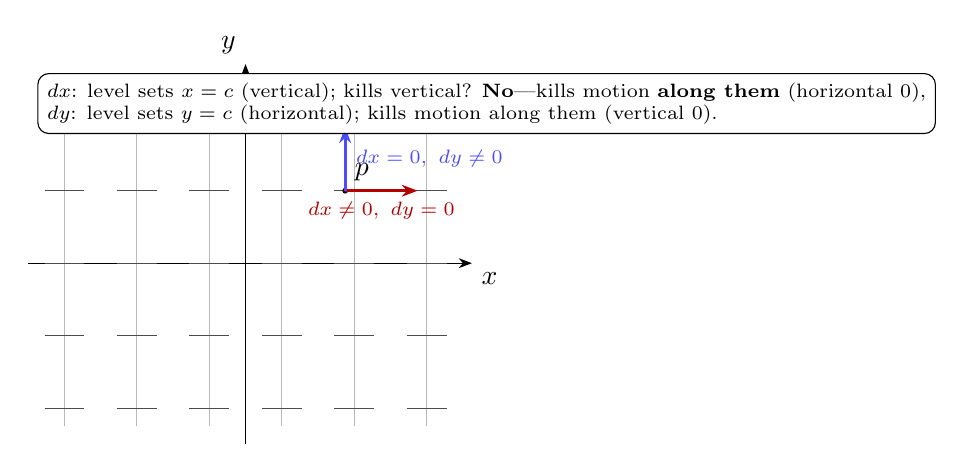
\begin{tikzpicture}[scale=1.15, >=Stealth]
		% Axes
		\draw[->] (-2.4,0) -- (2.5,0) node[below right] {$x$};
		\draw[->] (0,-2.0) -- (0,2.2) node[above left] {$y$};
		
		% Level sets of x=c (vertical lines) and dy's linelets (horizontal)
		% dx: linelets parallel to x=c (vertical lines) -> draw small vertical segments
		\foreach \X in {-2,-1.2,-0.4,0.4,1.2,2}{
			\draw[gray!55] (\X,-1.8) -- (\X,1.8);
		}
		% dy: linelets parallel to y=c (horizontal lines)
		\foreach \x in {-2.0,-1.2,-0.4,0.4,1.2,2.0}{
			\foreach \y in {-1.6,-0.8,0,0.8,1.6}{
				\draw[black!70, line width=0.35pt] (\x-0.22,\y) -- (\x+0.22,\y); % dy-glyphs (horizontal)
			}
		}
		% Mark a point and show what dx,dy measure
		\coordinate (p) at (1.1,0.8);
		\fill (p) circle (0.9pt) node[above right] {$p$};
		\draw[very thick, red!70!black, -{Stealth[length=2mm]}] (p) -- ++(0.8,0.0)
		node[midway, below, font=\scriptsize] {$dx\neq 0,\ dy=0$};
		\draw[very thick, blue!70, -{Stealth[length=2mm]}] (p) -- ++(0.0,0.7)
		node[midway, right, font=\scriptsize] {$dx=0,\ dy\neq 0$};
		
		\node[draw, rounded corners, fill=white, font=\scriptsize, align=left, anchor=north west]
		at (-2.3,2.1)
		{$dx$: level sets $x=c$ (vertical); kills vertical? \emph{No}—kills motion \emph{along them} (horizontal $0$),\\
			$dy$: level sets $y=c$ (horizontal); kills motion along them (vertical $0$).};
	\end{tikzpicture}
\end{center}

\subsection*{(b) Polar: $dr$ and $d\theta$}
\begin{center}
	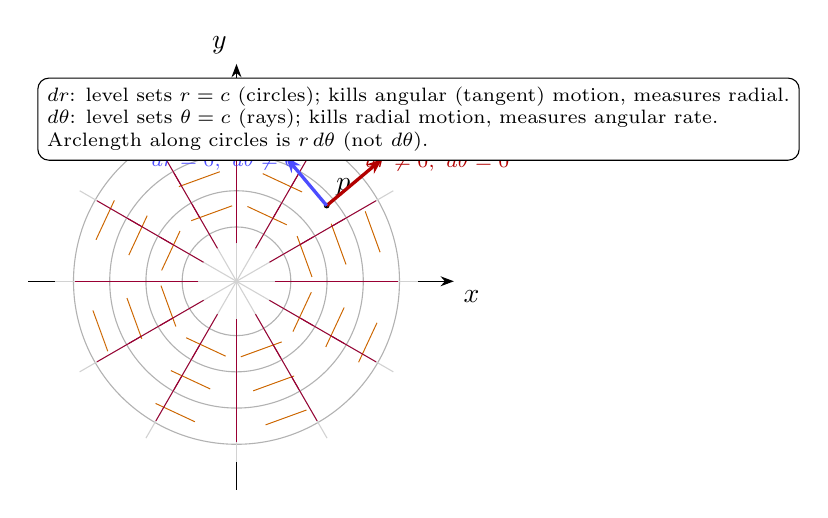
\begin{tikzpicture}[scale=1.15, >=Stealth]
		% Axes
		\draw[->] (-2.3,0) -- (2.4,0) node[below right] {$x$};
		\draw[->] (0,-2.3) -- (0,2.4) node[above left] {$y$};
		
		% Circles r=const (level sets of r)
		\foreach \R in {0.6,1.0,1.4,1.8}{
			\draw[gray!60] (0,0) circle (\R);
		}
		% Rays theta = const (level sets of theta)
		\foreach \ang in {0,30,60,90,120,150,180,210,240,270,300,330}{
			\draw[gray!35] (0,0) -- ({2.0*cos(\ang)},{2.0*sin(\ang)});
		}
		
		% dr glyphs: small segments tangent to circles (kill tangential motion? d r kills tangent → linelets tangent)
		\foreach \ang in {20,65,110,155,200,245,290,335}{
			\foreach \rad in {0.8,1.2,1.6}{
				% tangent direction is rotated +90 from radial direction
				\pgfmathsetmacro{\tx}{0.24*cos(\ang+90)}
				\pgfmathsetmacro{\ty}{0.24*sin(\ang+90)}
				\pgfmathsetmacro{\cx}{\rad*cos(\ang)}
				\pgfmathsetmacro{\cy}{\rad*sin(\ang)}
				\draw[orange!80!black, line width=0.35pt] (\cx-\tx,\cy-\ty) -- (\cx+\tx,\cy+\ty);
			}
		}
		
		% dtheta glyphs: small segments along rays (parallel to theta=const)
		\foreach \ang in {0,30,60,90,120,150,180,210,240,270,300,330}{
			\foreach \rad in {0.7,1.1,1.5}{
				\pgfmathsetmacro{\dx}{0.28*cos(\ang)}
				\pgfmathsetmacro{\dy}{0.28*sin(\ang)}
				\pgfmathsetmacro{\cx}{\rad*cos(\ang)}
				\pgfmathsetmacro{\cy}{\rad*sin(\ang)}
				\draw[purple!80!black, line width=0.35pt] (\cx-\dx,\cy-\dy) -- (\cx+\dx,\cy+\dy);
			}
		}
		
		% A point p and two small motions: radial and angular
		\coordinate (p) at ({1.3*cos(40)},{1.3*sin(40)});
		\fill (p) circle (0.9pt) node[above right] {$p$};
		% radial motion (dr ≠ 0, dθ = 0)
		\draw[very thick, red!70!black, -{Stealth[length=2mm]}]
		(p) -- ++({0.8*cos(40)},{0.8*sin(40)})
		node[midway, above right, font=\scriptsize] {$dr\neq 0,\ d\theta=0$};
		% angular motion (dr = 0, dθ ≠ 0) -- tangent to circle
		\draw[very thick, blue!70, -{Stealth[length=2mm]}]
		(p) -- ++({-0.7*sin(40)},{0.7*cos(40)})
		node[midway, above left, font=\scriptsize] {$dr=0,\ d\theta\neq 0$};
		
		\node[draw, rounded corners, fill=white, font=\scriptsize, align=left, anchor=north west]
		at (-2.2,2.25)
		{$dr$: level sets $r=c$ (circles); kills angular (tangent) motion, measures radial.\\
			$d\theta$: level sets $\theta=c$ (rays); kills radial motion, measures angular rate.\\
			Arclength along circles is $r\,d\theta$ (not $d\theta$).};
	\end{tikzpicture}
\end{center}


\newpage
\section*{Big picture mappings}
\begin{itemize}
	\item \textbf{Variable \(\;x\;\to\;dx\)} (small change): If \(x\) is a coordinate on \(\R\) (or part of a coordinate chart),
	then \(dx\) is its \emph{differential}—a linear map that takes a tangent vector (an infinitesimal displacement)
	and returns the rate of change of \(x\) along that displacement. Formally, \(dx\in T_p^*M\) is a covector.
	
	\item \textbf{Scalar field \(\;f\;\to\;df\)} (covector field): A smooth \(f:M\to\R\) determines its \emph{differential}
	\(df\), a \emph{1-form} (covector field) defined pointwise by
	\[
	df_p(v)\;=\;\left.\frac{d}{dt}\right|_{t=0} f(\gamma(t)),\quad \gamma(0)=p,\ \dot\gamma(0)=v.
	\]
	In coordinates \(x^1,\dots,x^n\), \(df=\sum_i \frac{\partial f}{\partial x^i}\,dx^i\).
	
	\item \textbf{Function \(\;f\;\to\;\) level sets}: For each constant \(c\in\R\), the \emph{level set}
	\(f^{-1}(c)=\{p\in M:\ f(p)=c\}\) collects points where \(f\) has the same value.
	When \(\nabla f\neq0\), level sets are hypersurfaces orthogonal (via a metric) to \(\nabla f\).
	
	\item \textbf{0-form \(\;\to\;\) 1-form}: A smooth function \(f\) is a \emph{0-form}. Its exterior derivative \(d\)
	sends 0-forms to 1-forms: \(d:\Omega^0(M)\to\Omega^1(M)\), namely \(f\mapsto df\).
\end{itemize}

\section*{Concrete example on \(\R^2\)}
Let \(f(x,y)=x^2+y^2\).
\[
df \;=\; 2x\,dx + 2y\,dy,\qquad
\nabla f \;=\; (2x,2y) \quad \text{(Euclidean metric)}.
\]
At a point \(p=(x,y)\), for a small displacement \(v=(v_x,v_y)\),
\[
df_p(v) \;=\; 2x\,v_x + 2y\,v_y \;=\; \nabla f(p)\cdot v.
\]
Level sets are circles \(x^2+y^2=c\) (concentric about the origin). Tangent motion along a level set contributes
nothing to \(df\); only the component of motion across level sets (along the gradient) contributes.

\section*{One-line summary}
\[
\boxed{\ x \mapsto dx\ \text{(basis 1-forms)};\quad
	f \mapsto df\ \text{(1-form)};\quad
	f \mapsto \{f=c\}\ \text{(level sets)};\quad
	0\text{-form} \xrightarrow{\,d\,} 1\text{-form}\ }.
\]

\bigskip\hrule\bigskip

\section*{Tiny TikZ sketch (level sets and \(df\))}
\begin{center}
	\begin{tikzpicture}[scale=1.25, >=Stealth]
		% Axes
		\draw[->] (-2.2,0) -- (2.3,0) node[below right] {$x$};
		\draw[->] (0,-2.2) -- (0,2.3) node[above left] {$y$};
		
		% Level sets (circles) for f(x,y)=x^2+y^2
		\foreach \r in {0.8,1.2,1.6,2.0}{
			\draw[gray!65] (0,0) circle (\r);
		}
		\node[gray!60, font=\scriptsize] at (1.9,0.18) {$f=\text{const}$};
		
		% Pick a point p and draw gradient (normal) and a tangent
		\coordinate (p) at (1.1,0.9);
		\fill (p) circle (1.0pt) node[above right] {$p$};
		
		% Gradient ~ (2x,2y) scaled visually
		\coordinate (gTip) at ($(p) + (0.9*2*1.1,0.9*2*0.9)$);
		\draw[very thick, red!75!black, -{Stealth[length=2.2mm]}] (p) -- (gTip)
		node[above right, xshift=2pt, font=\scriptsize] {$\nabla f$ (normal)};
		
		% Tangent direction (perp to gradient)
		\coordinate (tTip) at ($(p) + (-0.85,0.85)$);
		\draw[very thick, blue!70, -{Stealth[length=2.0mm]}] (p) -- (tTip)
		node[above left, font=\scriptsize] {tangent};
		
		% Annotation for df
		\node[draw, rounded corners, fill=white, align=left, font=\scriptsize, anchor=north west]
		at (-2.1,2.25)
		{$f(x,y)=x^2+y^2$\\[2pt]
			$df=2x\,dx+2y\,dy$ (1-form)\\[2pt]
			$df_p(v)=\nabla f(p)\!\cdot v$\\
			tangent $\Rightarrow 0$, normal $\Rightarrow$ measured.};
	\end{tikzpicture}
\end{center}


\newpage
\section{Zero Curl and Closed}
%In $\R^3$, the \textbf{curl} of a vector field $\vec F = \begin{bmatrix}
%	P & Q & R
%\end{bmatrix}^{\top}$ measures its local ``swirl'' or rotation.
%\[\nabla \times \F = \vect{\pderiv{R}{y} - \pderiv{Q}{z} \\[1ex] \pderiv{P}{z} - \pderiv{R}{x} \\[1ex] \pderiv{Q}{x} - \pderiv{P}{y}} \]
\end{document}
